\section{R\'esum\'e en fran\c cais}
%-----------------------------------------------------------------------------
%-----------------------------------------------------------------------------
%-----------------------------------------------------------------------------
\subsection*{Introduction}
\begin{figure}
	{\centering
		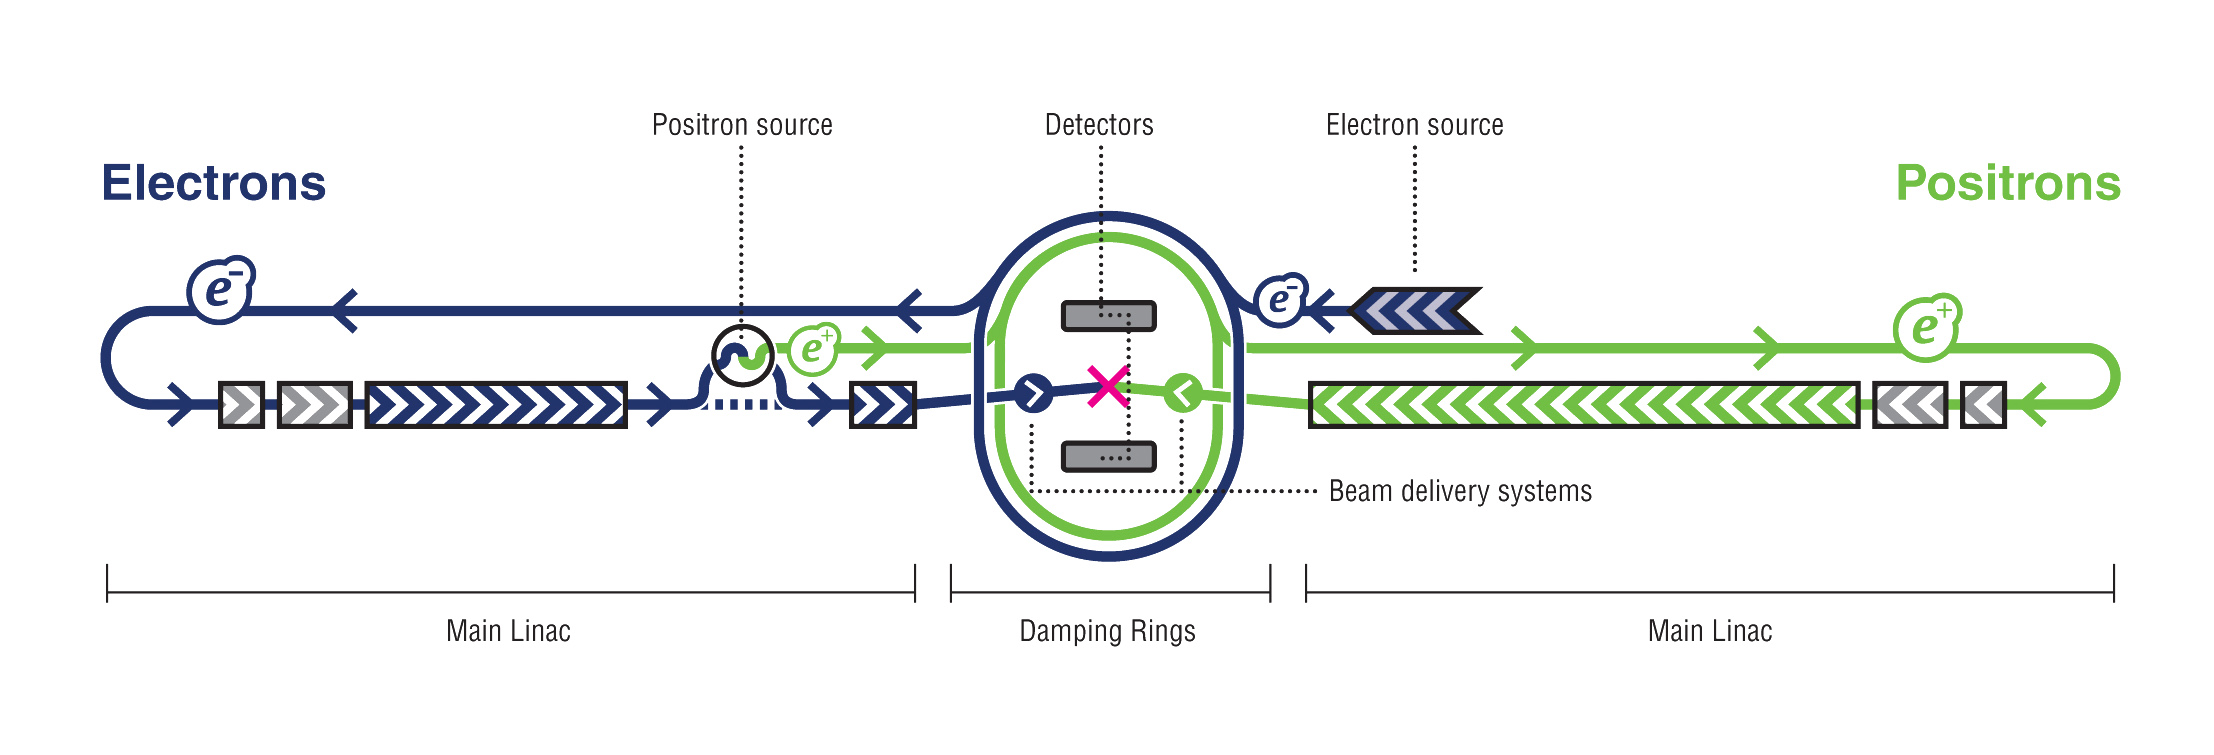
\includegraphics[width=0.95\textwidth]{graphics/ILC_scheme.jpg}
		\caption{\sl Vue sch\'ematique de l'ILC.}
		\label{fig:ILCSchemeF}
	}
\end{figure}

\begin{figure}
	\centering
	\begin{subfigure}{0.5\textwidth}
		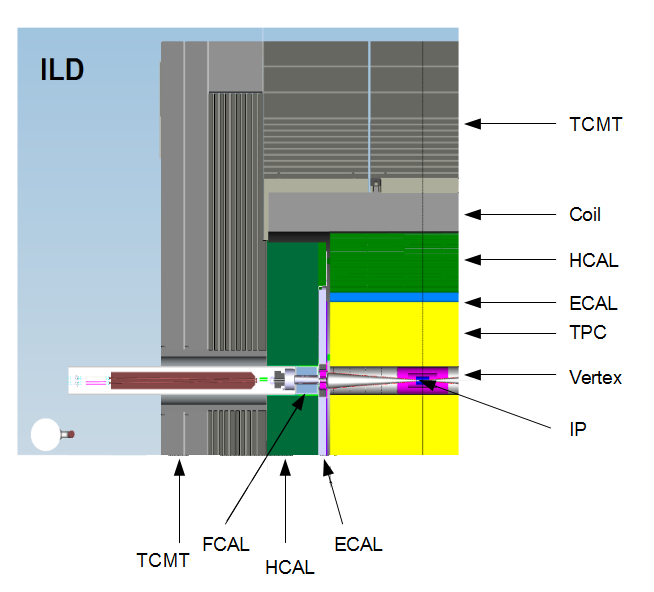
\includegraphics[width=0.95\textwidth]{graphics/ILD.png}
		
	\end{subfigure}% 
	\begin{subfigure}{0.5\textwidth}
		\centering
		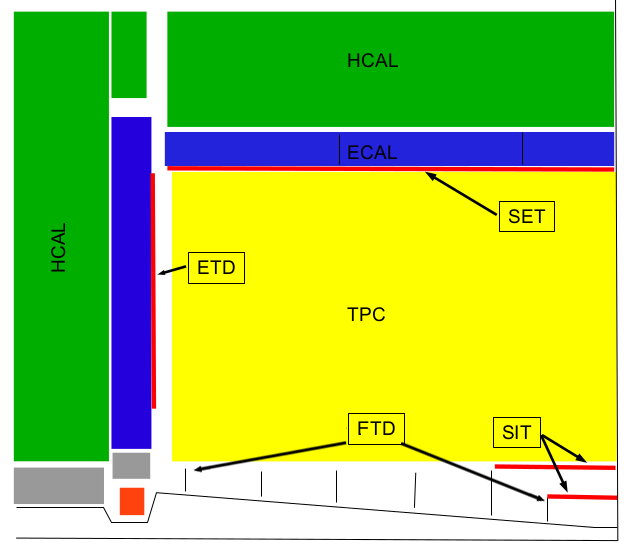
\includegraphics[width=0.9\textwidth]{graphics/ILDtracking.png}
		
	\end{subfigure}
	\caption{\sl Gauche: Vue sch\'ematique de l'ILD. Droite: Zoom sur les détecteurs internes.}
	\label{fig:ILDSchemeF}
\end{figure}
%-----------------------------------------------------------------------------
%-----------------------------------------------------------------------------
%-----------------------------------------------------------------------------
\subsection*{Calorim\`etre \'electromagn\'etique silicium-tungst\`ene hautement granulaire}

\begin{figure}[H]
	\centering
	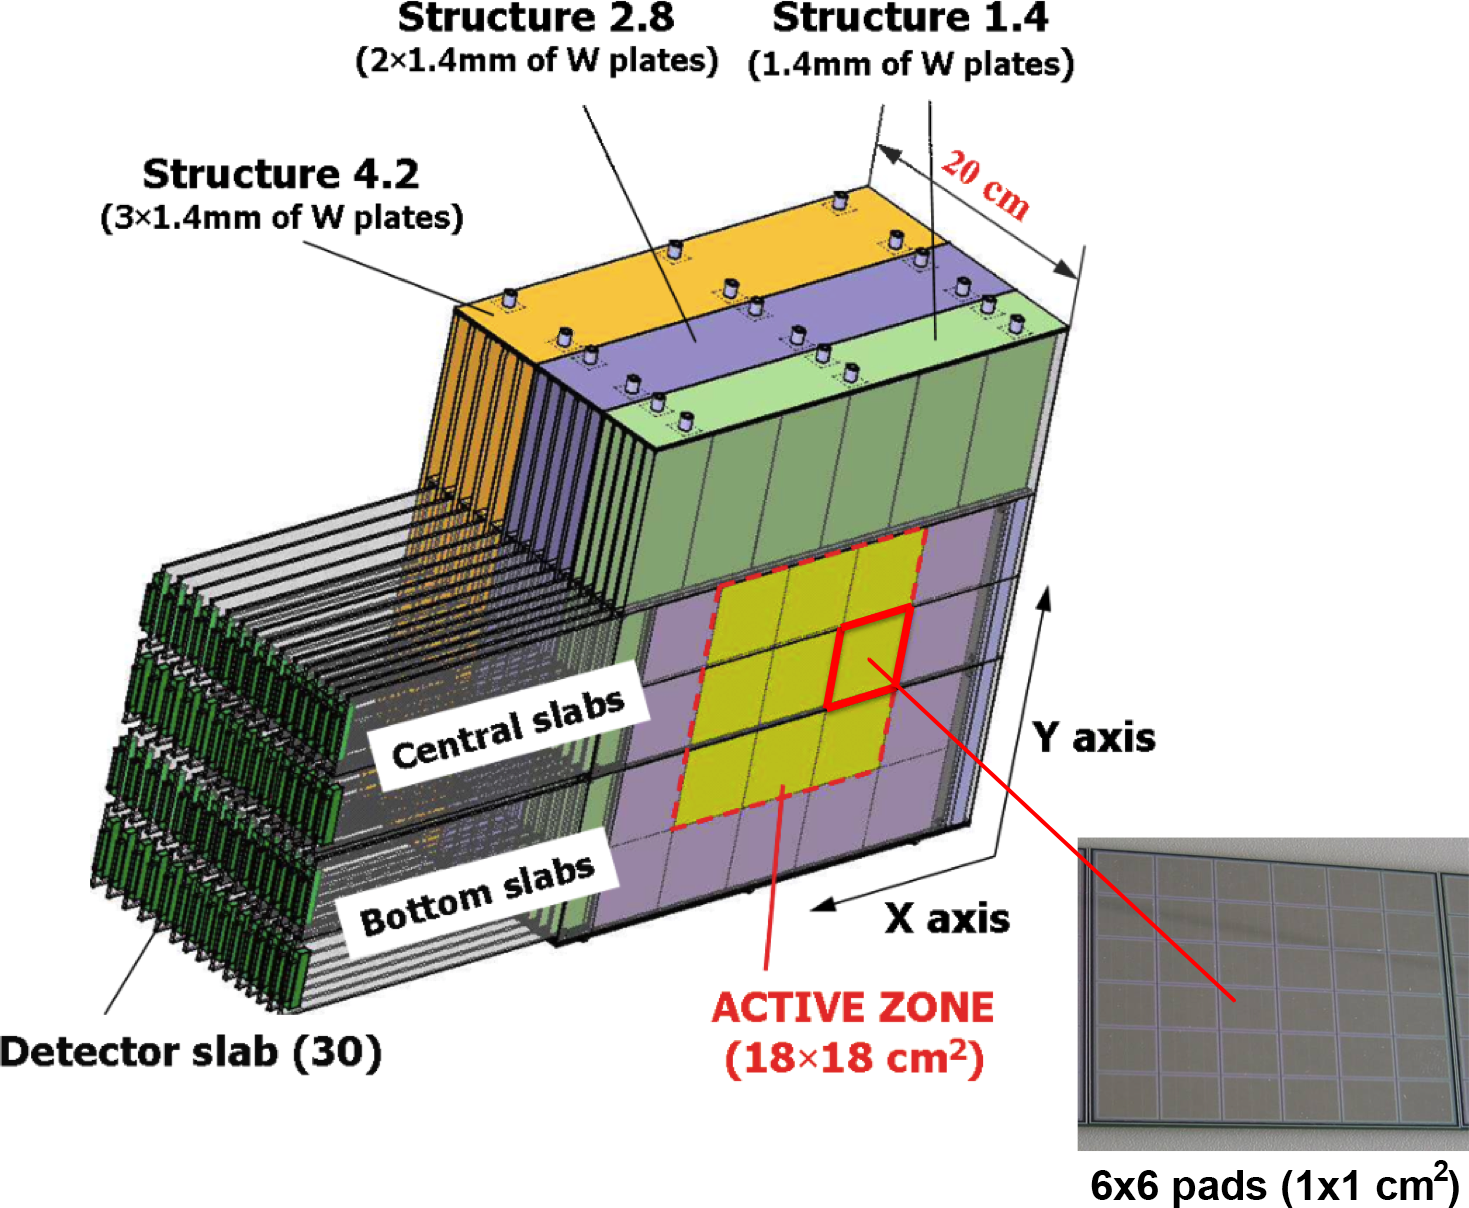
\includegraphics[width=0.55\textwidth]{ECAL/graphics/ecal-new.png}
	\caption{\label{fig:ECAL-schemeF} \sl  Vue sch\'ematique de \ecal.}
\end{figure}

%-----------------------------------------------------------------------------
%-----------------------------------------------------------------------------
%-----------------------------------------------------------------------------
\subsection*{L'algorithme de reconstruction des traces}

\begin{figure}
	\centering
	\begin{subfigure}{0.5\textwidth}
		\centering
		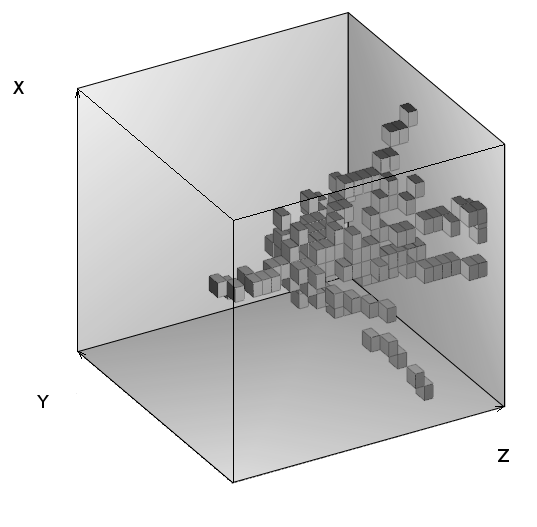
\includegraphics[width=.90\linewidth]{ECAL/graphics/before.png}
		\caption{\label{fig:beforeF} \sl avec région d'interaction.}
	\end{subfigure}% 
	\begin{subfigure}{0.5\textwidth}
		\centering
		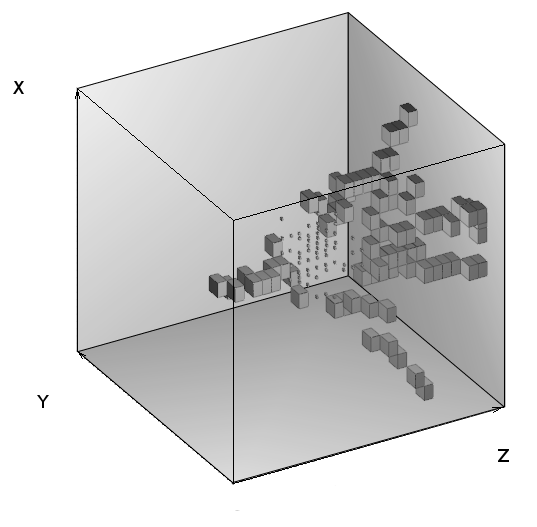
\includegraphics[width=.90\linewidth]{ECAL/graphics/after2.png}
		\caption{\label{fig:afterF} \sl sans région d'interaction.}
	\end{subfigure}
	\caption{ \sl Visualisation d'événement de l'interaction pion primaire avec 10\,GeV d'energie enregistré au FNAL 2008 avant \textit{(a)} et apr\'es suppression de la région d'interaction\textit{(b)}. }
	%Event 16-17 in Data10.root
	\label{fig:testF}
\end{figure}


\begin{figure}
	\centering
	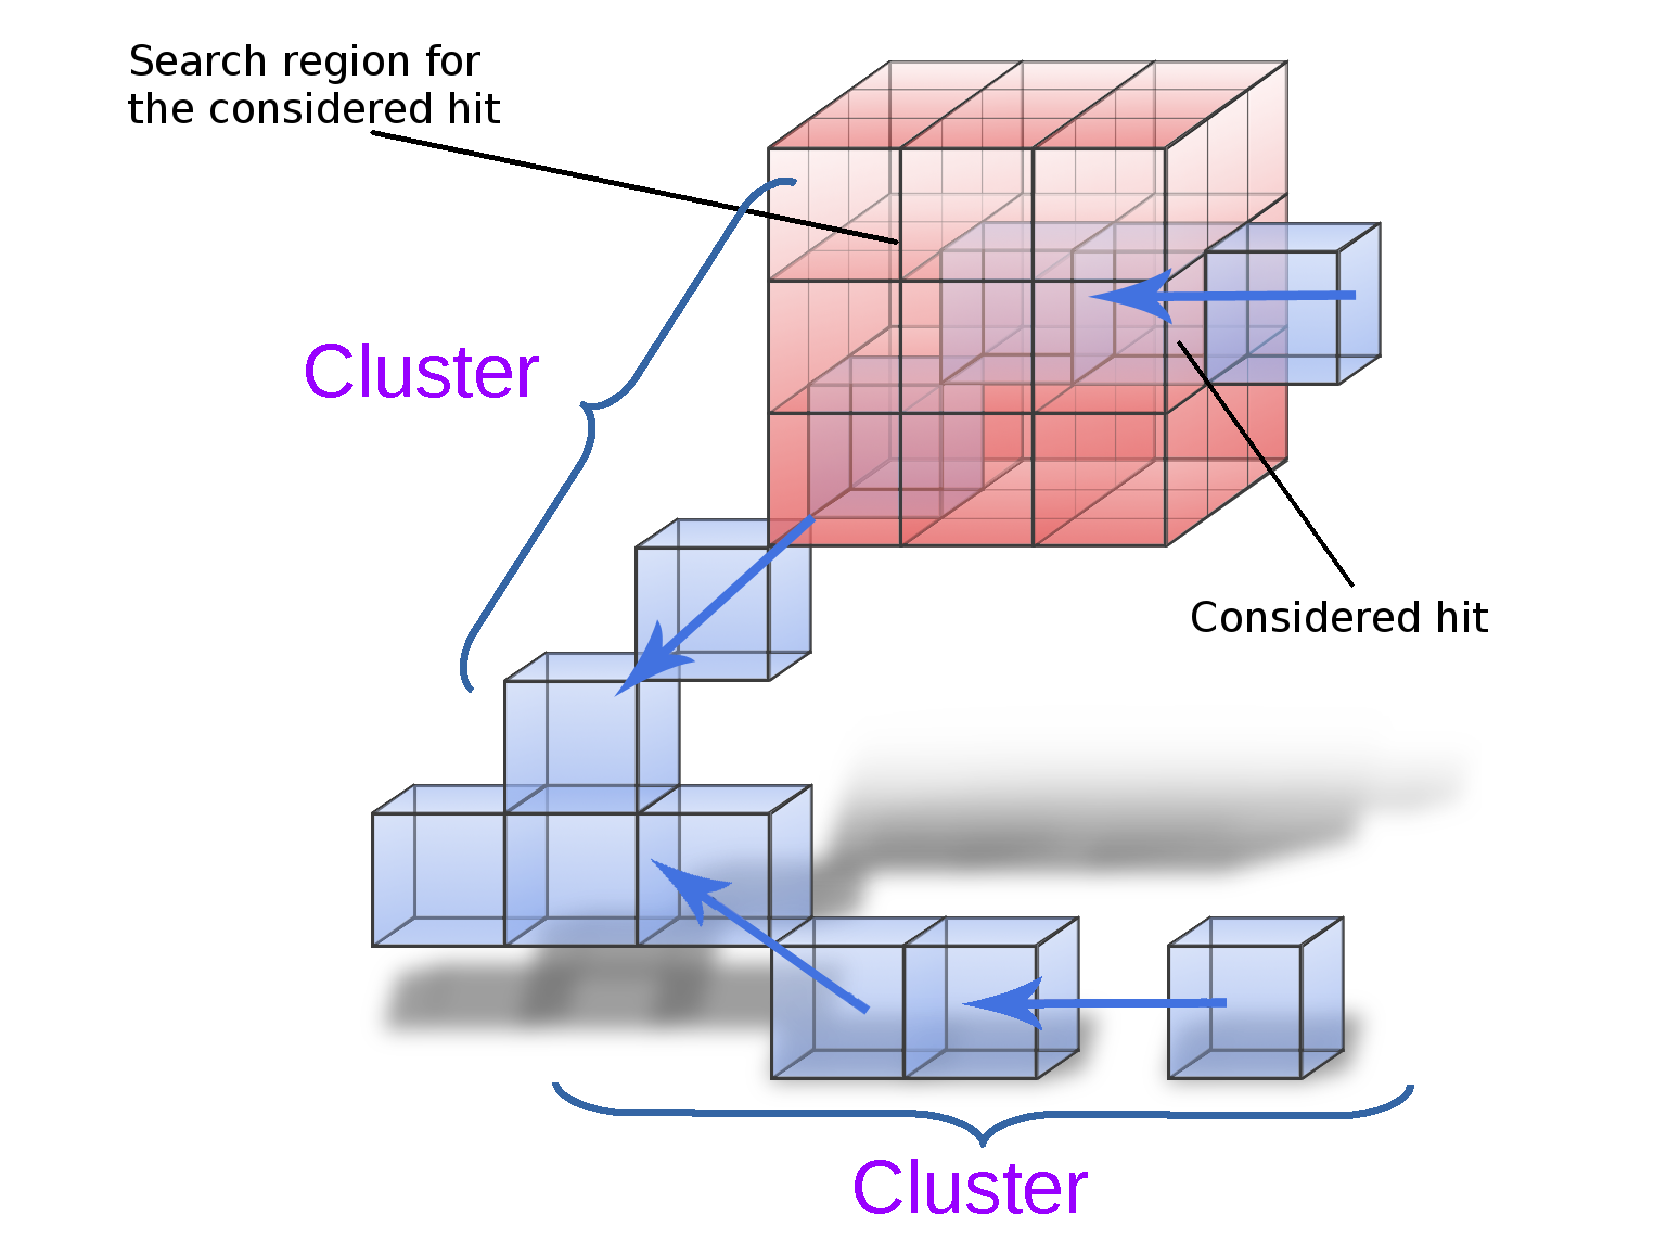
\includegraphics[width=0.55\textwidth]{ECAL/graphics/demo-v3.pdf}
	\caption{\label{fig:democlusterF} \sl Illustration de l'étape de clusterization. Les pixels actives sont représentés par des cubes bleus, et la zone de recherche pour les impacts adjacents est indiquée par des cubes rouges. Les flèches bleues indiquent la direction du flux de clusterization.}
\end{figure}

%-----------------------------------------------------------------------------
%-----------------------------------------------------------------------------
%-----------------------------------------------------------------------------

\subsection*{Comparaison des simulations avec les données réelles}



\begin{figure}
	\centering
	\begin{subfigure}{0.5\textwidth}
		\centering
		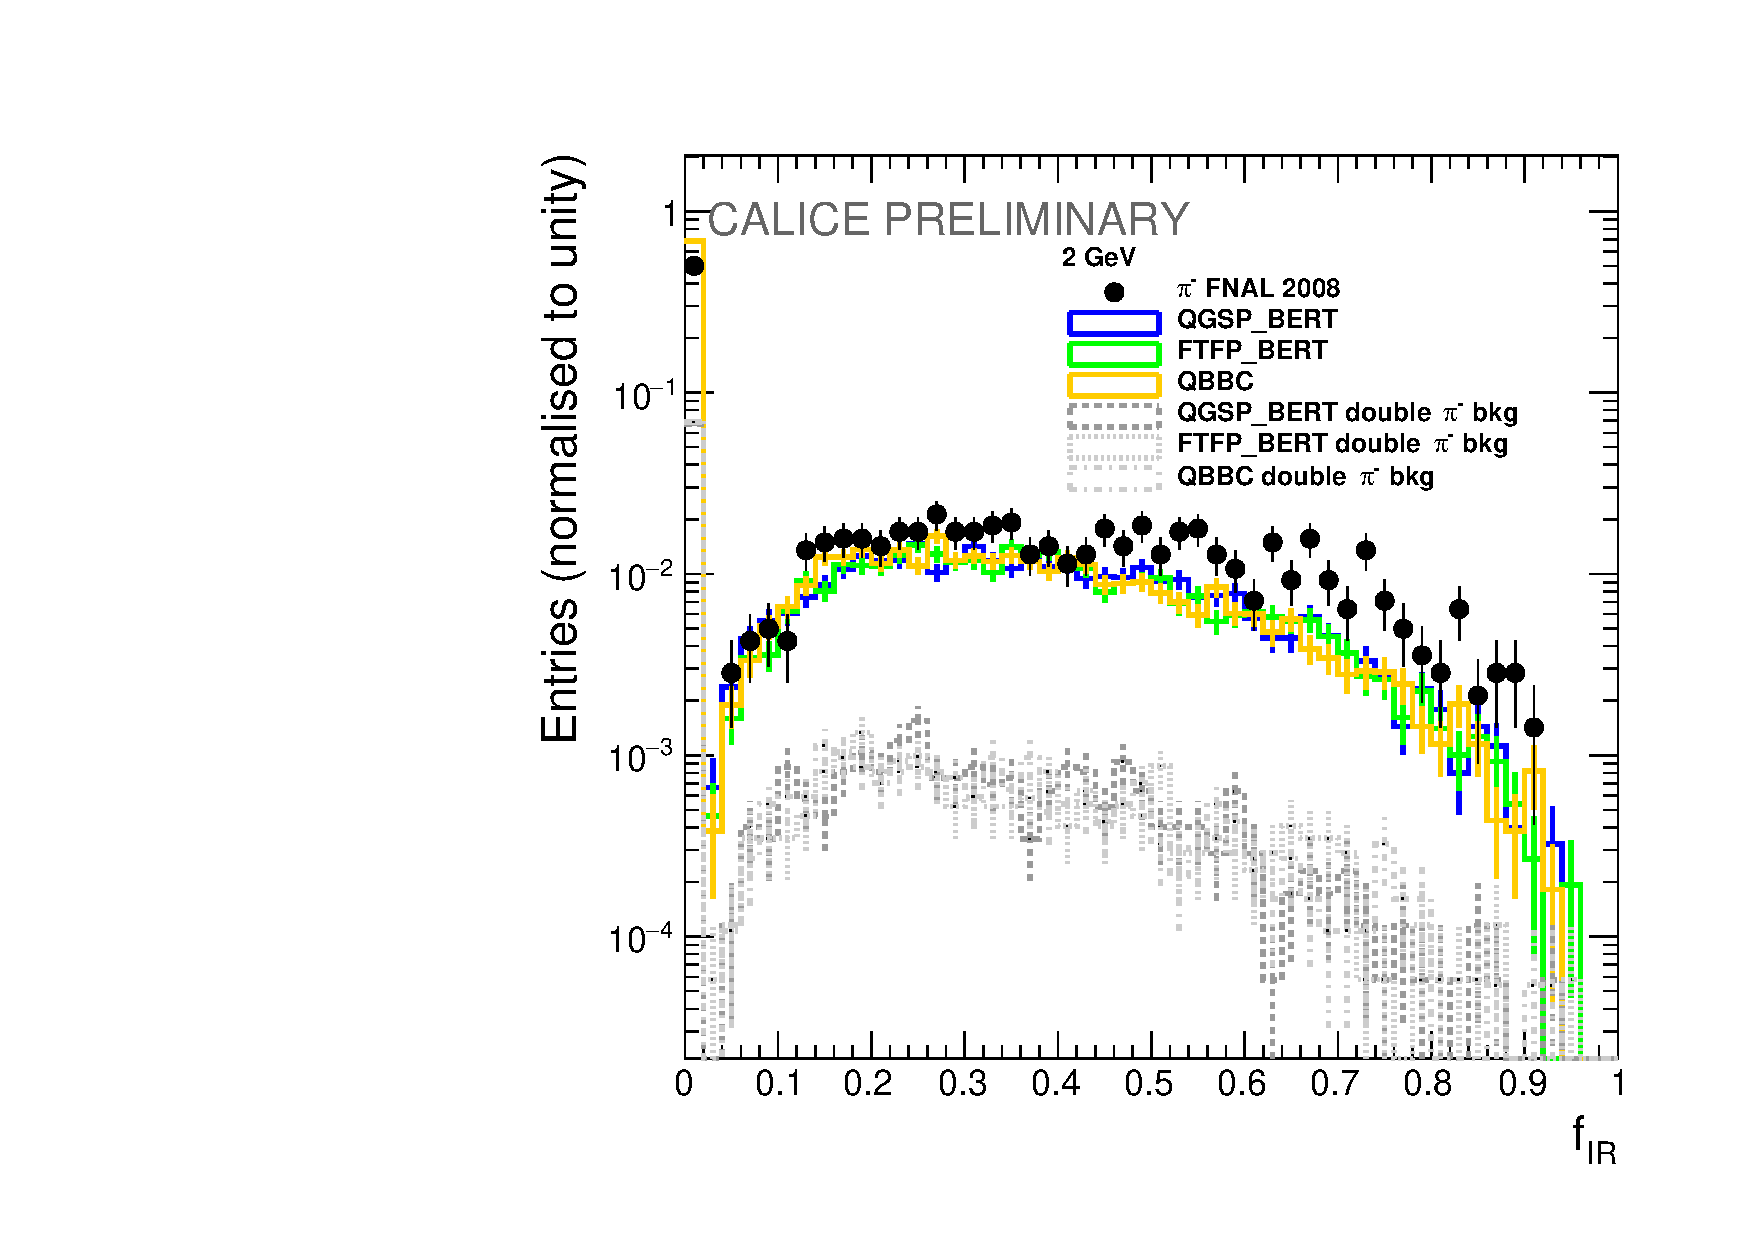
\includegraphics[width=.90\linewidth]{ECAL/plots/e-ir-2.pdf}
		\caption{\label{fig:efr2F} }
	\end{subfigure}% 
	\begin{subfigure}{0.5\textwidth}
		\centering
		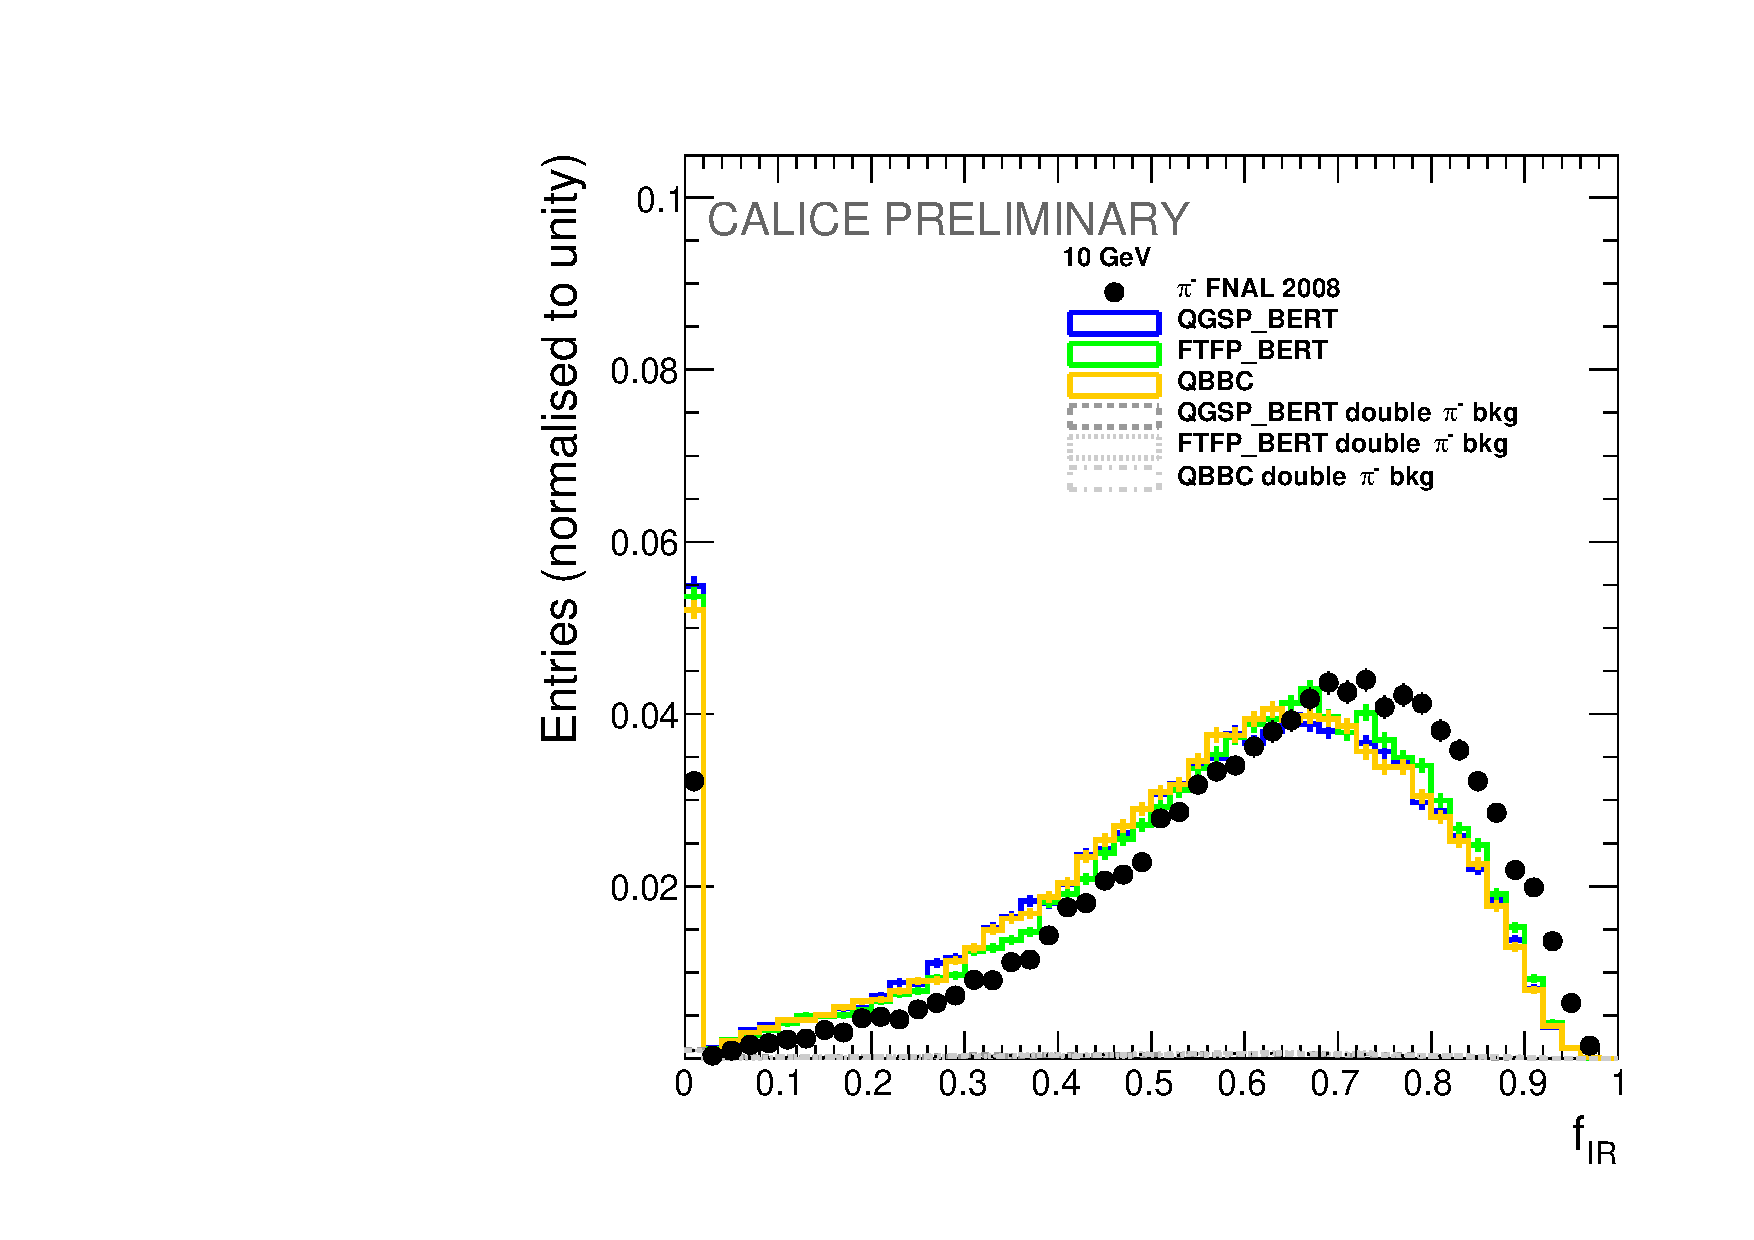
\includegraphics[width=.90\linewidth]{ECAL/plots/e-ir-10.pdf}
		\caption{\label{fig:efr10F} }
	\end{subfigure}
	\caption{\label{fig:irexampleF} \sl% {\bf Fig.~\ref{fig:efr2}: Remind me how the linear plot looks like} 
		Comparaison de $f_{IR}$ entre les données et les simulations pour trois {\sc Geant}4  listes physiques de l'\'energies 2 (a) et 10 (b) GeV de particule primordiale.}
\end{figure}

\begin{figure}
	\centering
	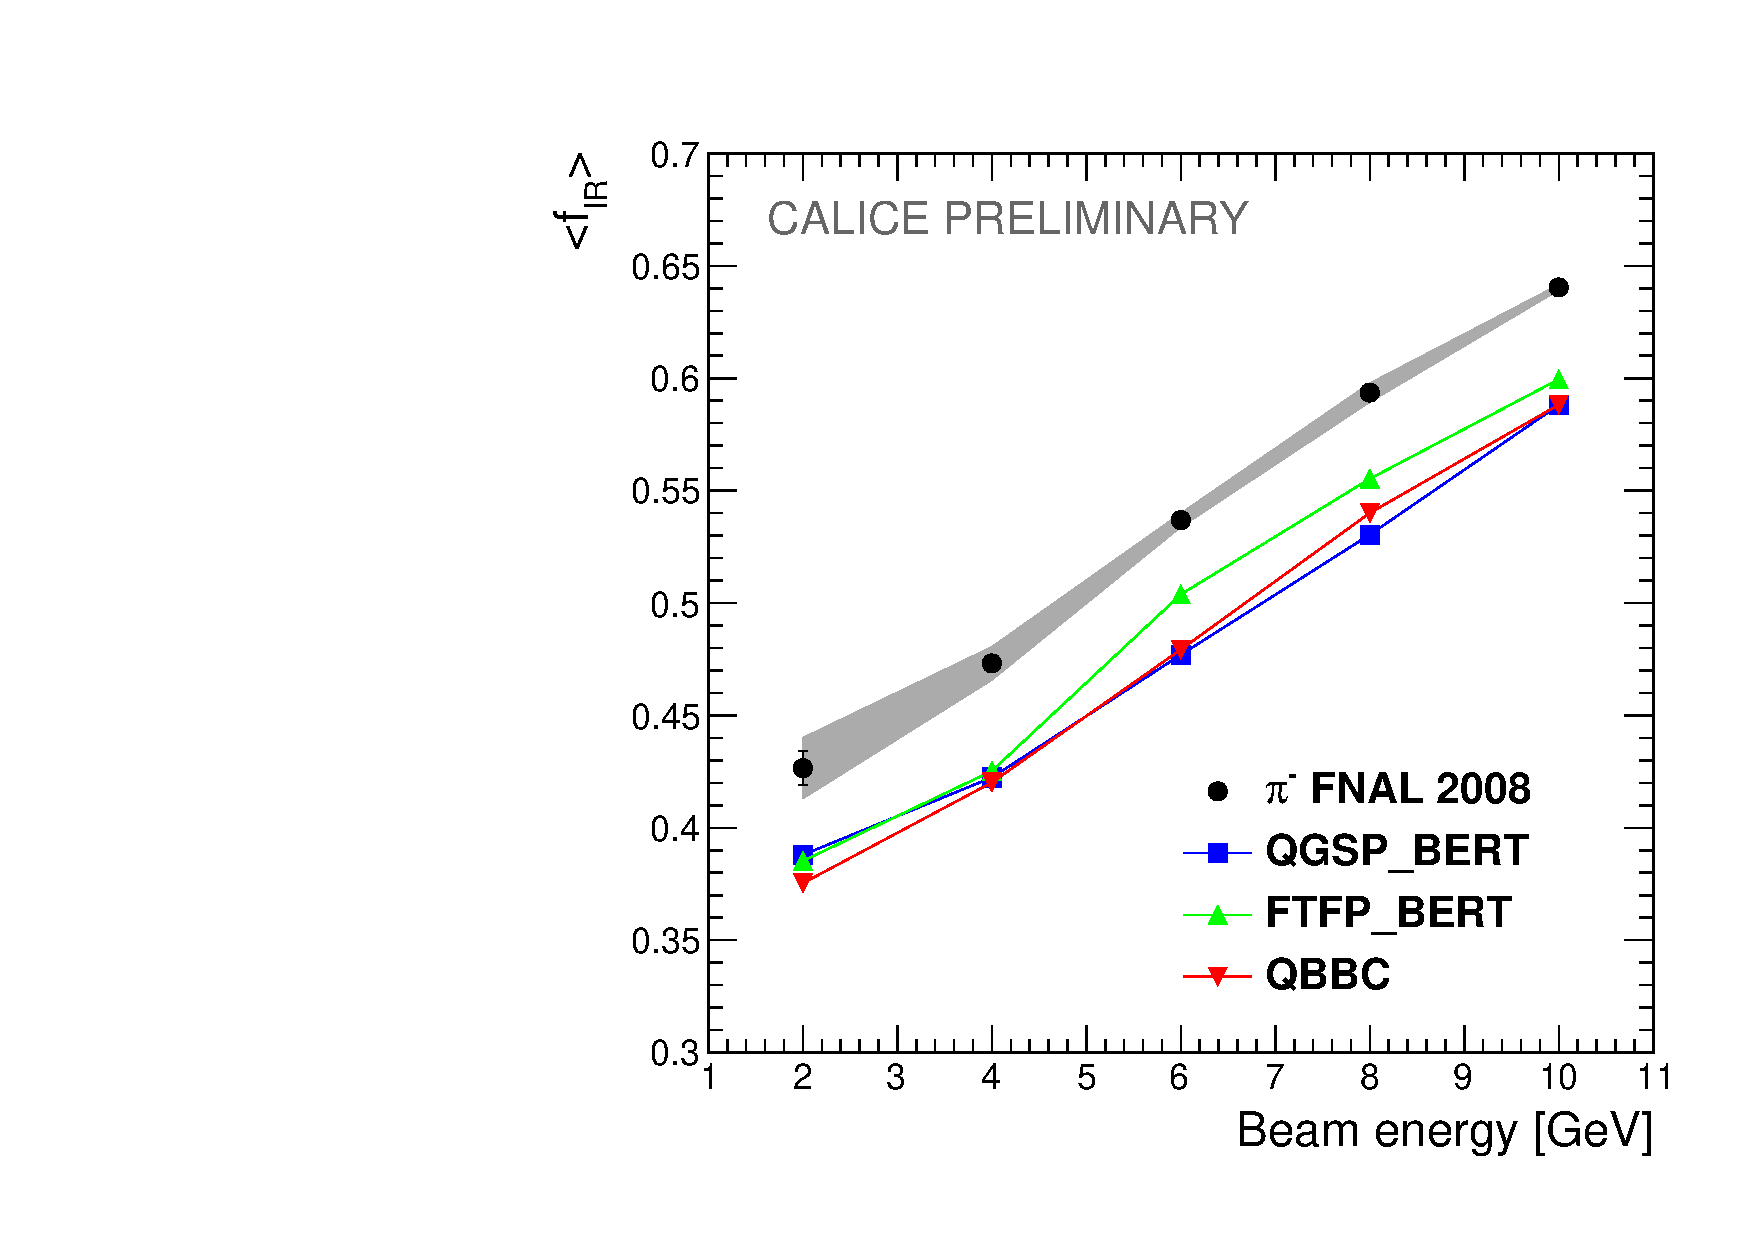
\includegraphics[width=0.5\textwidth]{ECAL/plots/e-ir-graph.pdf}
	\caption{\label{fig:irgraphF} \sl  Fraction moyenne du dépôt d'énergie dans la région d'interaction pour les données et les simulations  pour trois listes physiques \geant\ comme une fonction de l'énergie du faisceau (2 \, GeV à 10 \, GeV).}
\end{figure}

\begin{figure}
	\centering
	\begin{subfigure}{0.5\textwidth}
		\centering
		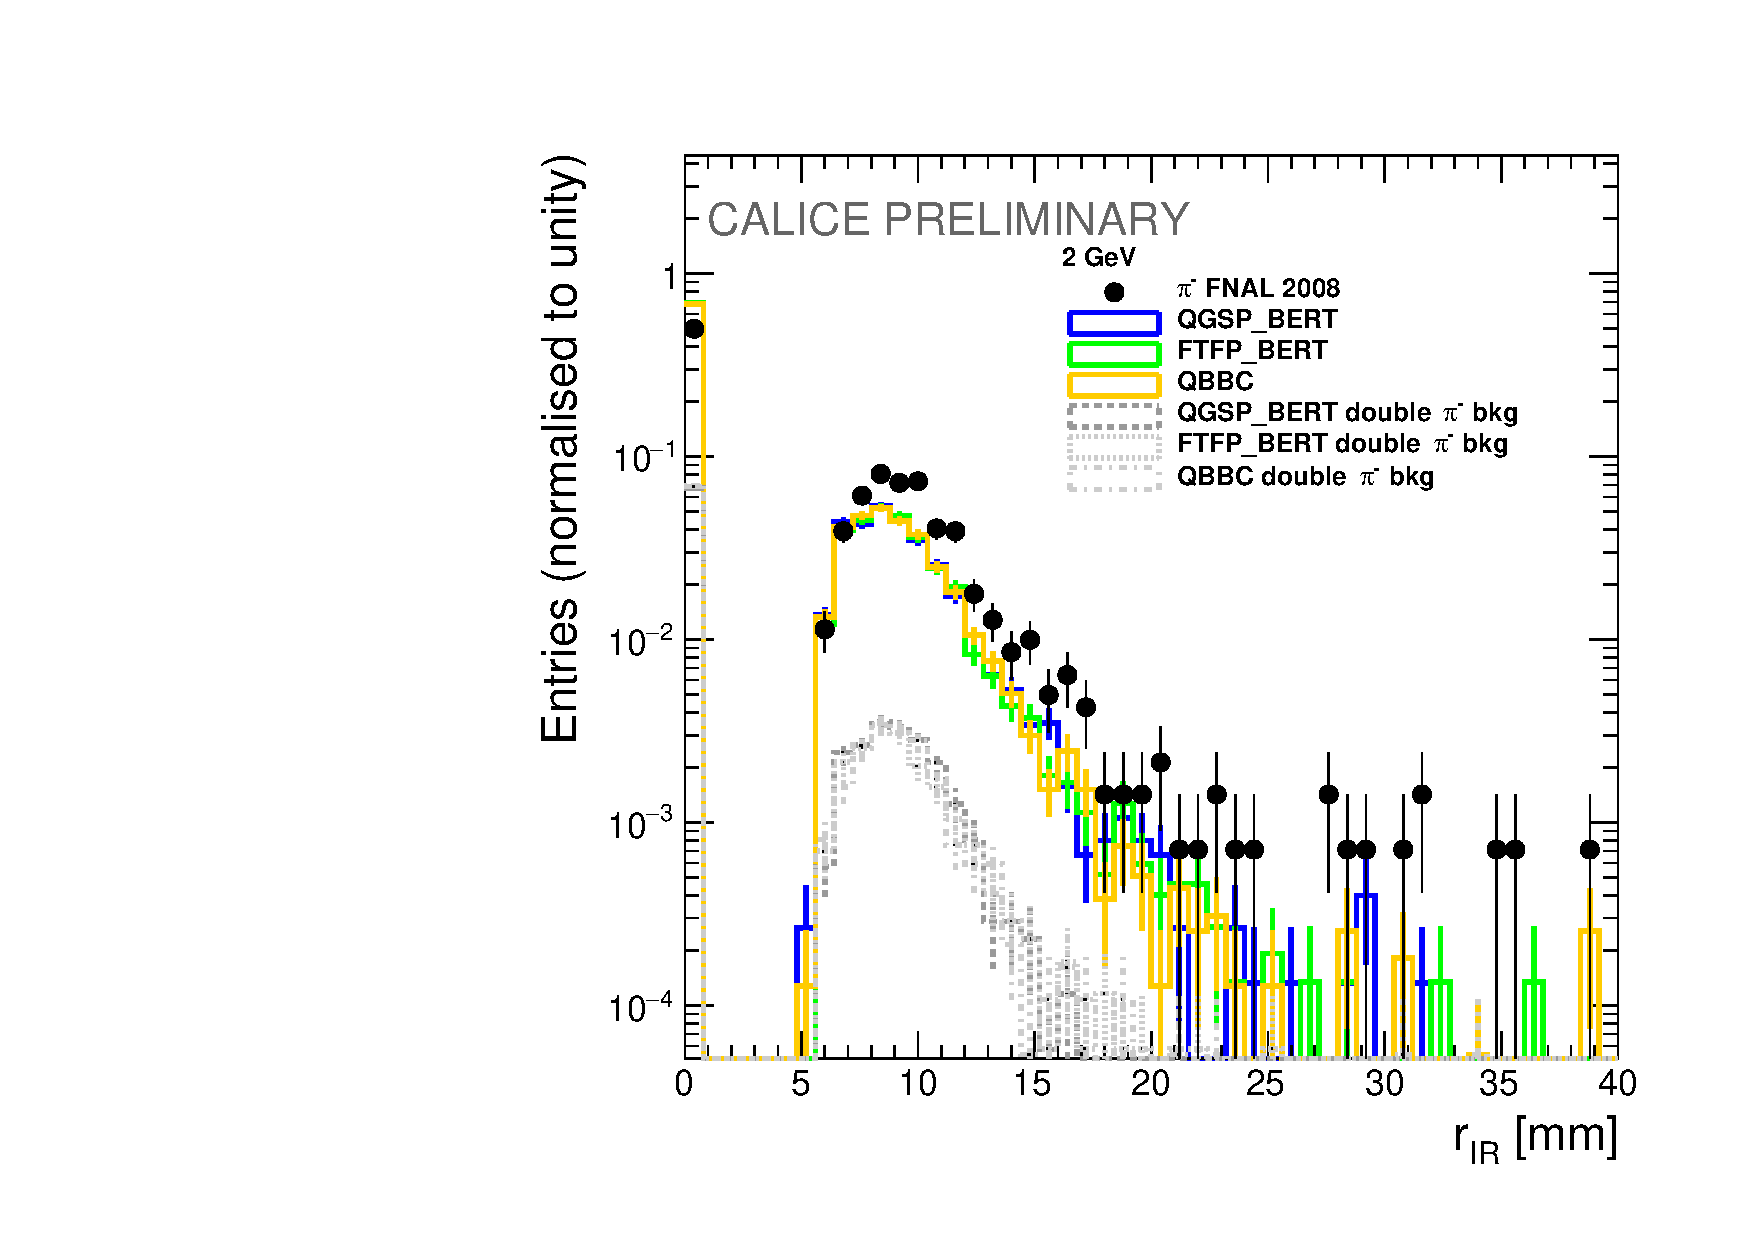
\includegraphics[width=.90\linewidth]{ECAL/plots/r-ir-2.pdf}
		\caption{\label{fig:rir2F} }
	\end{subfigure}% 
	\begin{subfigure}{0.5\textwidth}
		\centering
		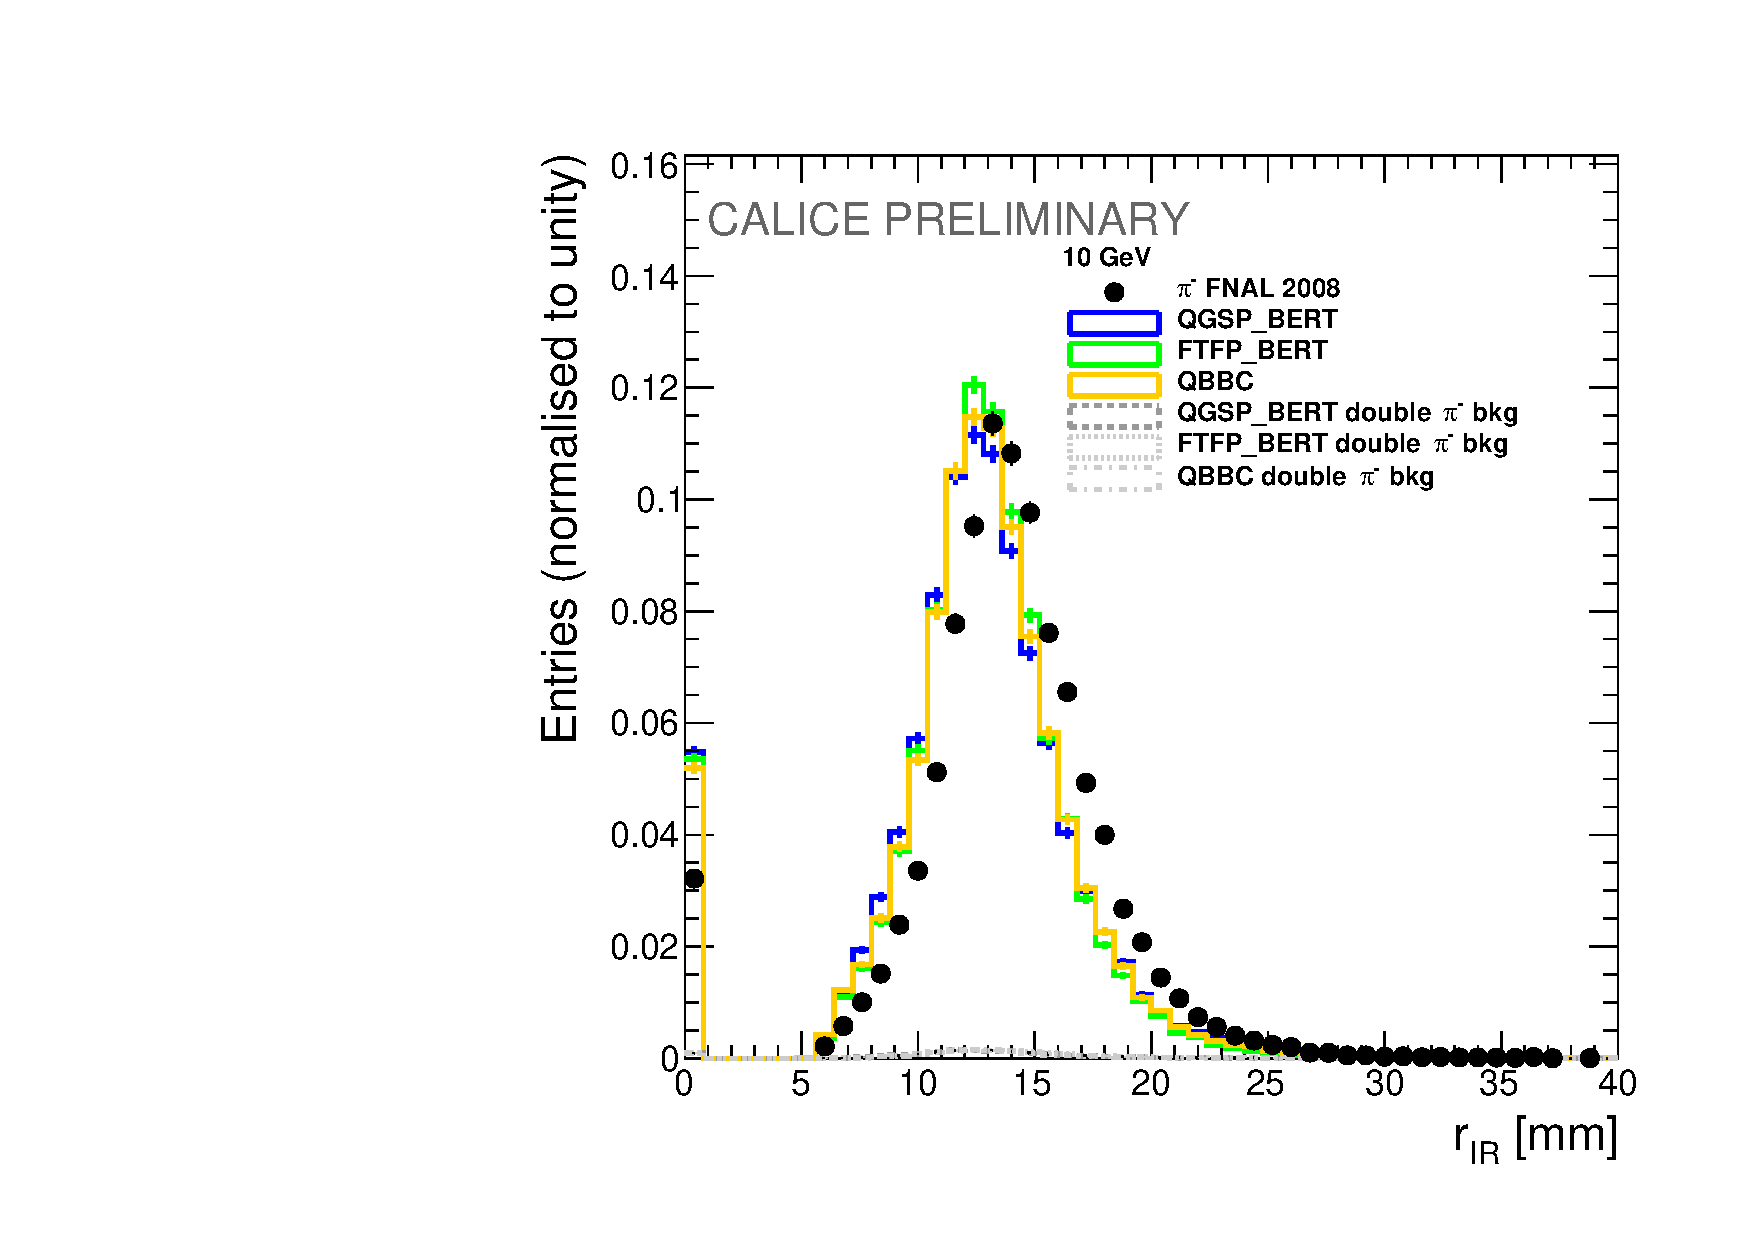
\includegraphics[width=.90\linewidth]{ECAL/plots/r-ir-10.pdf}
		\caption{\label{fig:rir10F} }
	\end{subfigure}
	\caption{\label{fig:rirexampleF} \sl %{\bf Same remark as for Fig.~\ref{fig:efr2} }
		Comparaison de $r_{IR}$ entre les données et les simulations pour trois {\sc Geant}4  listes physiques de l'\'energies 2 (a) et 10 (b) GeV de particule primordiale.}
\end{figure}

\begin{figure}
	\centering
	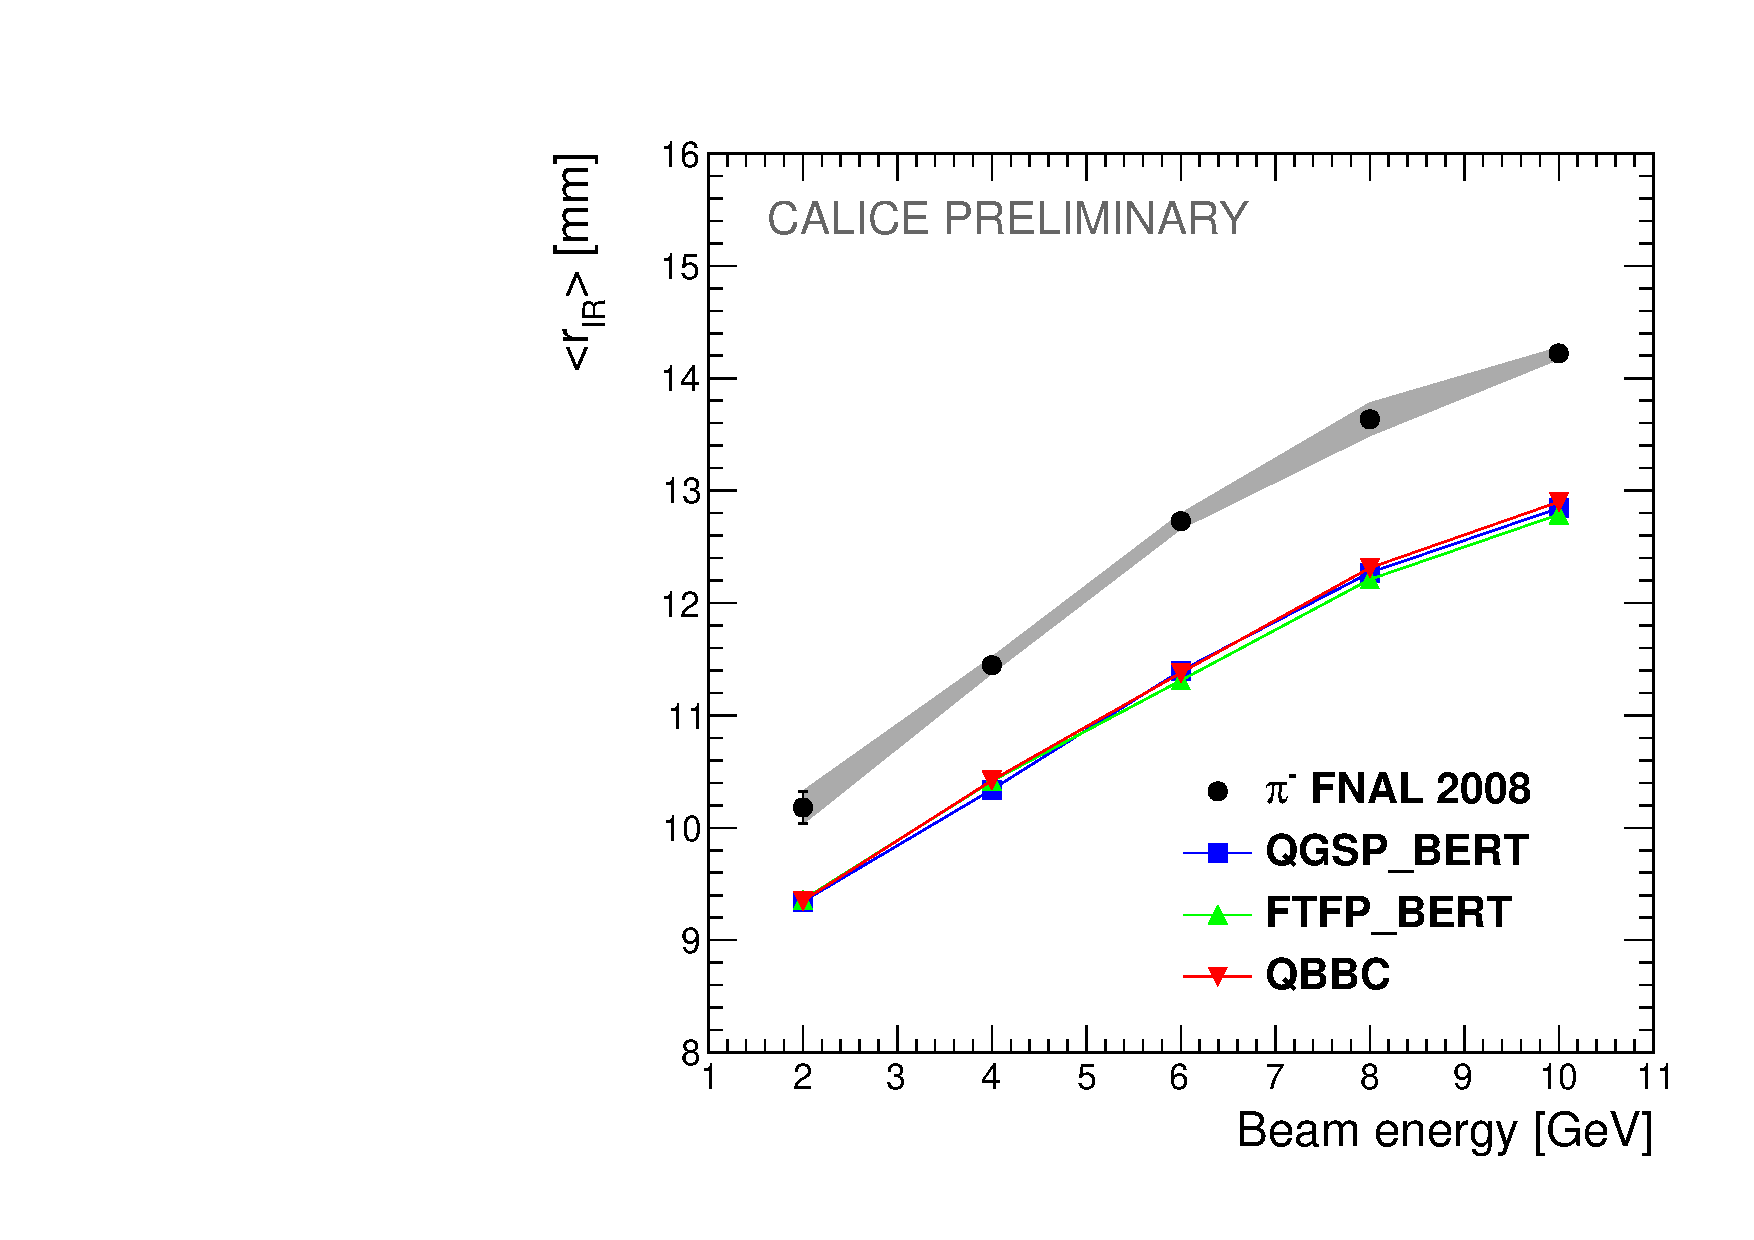
\includegraphics[width=0.5\textwidth]{ECAL/plots/r-ir-graph.pdf}
	\caption{\label{fig:irrgraphF} \sl Radius lateral moyen de la région d'interaction pour les données et les simulations  pour trois listes physiques \geant\ comme une fonction de l'énergie du faisceau (2 \, GeV à 10 \, GeV).}
\end{figure}

\begin{figure}
	\centering
	\begin{subfigure}{0.5\textwidth}
		\centering
		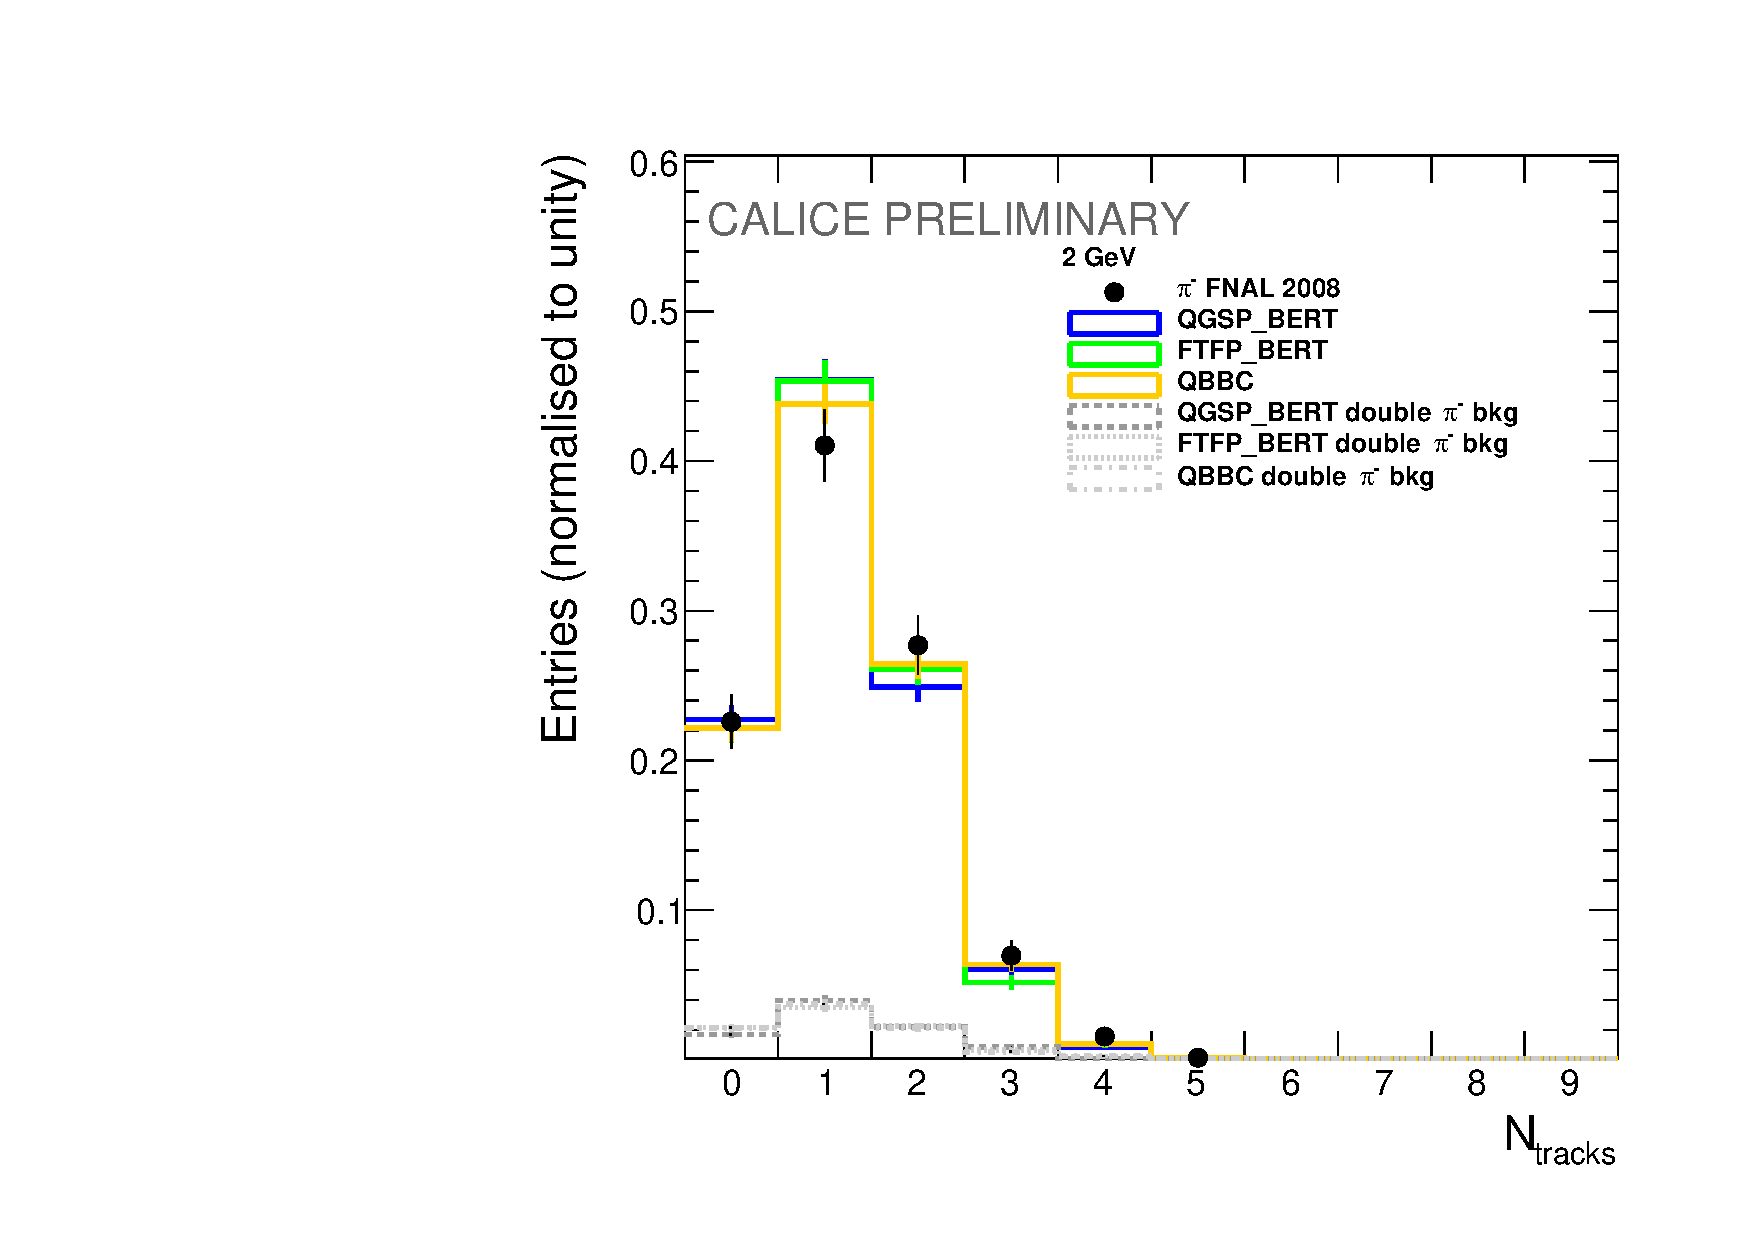
\includegraphics[width=.90\linewidth]{ECAL/plots/ntracks-2.pdf}
		\caption{\label{fig:tr2F} }
	\end{subfigure}% 
	\begin{subfigure}{0.5\textwidth}
		\centering
		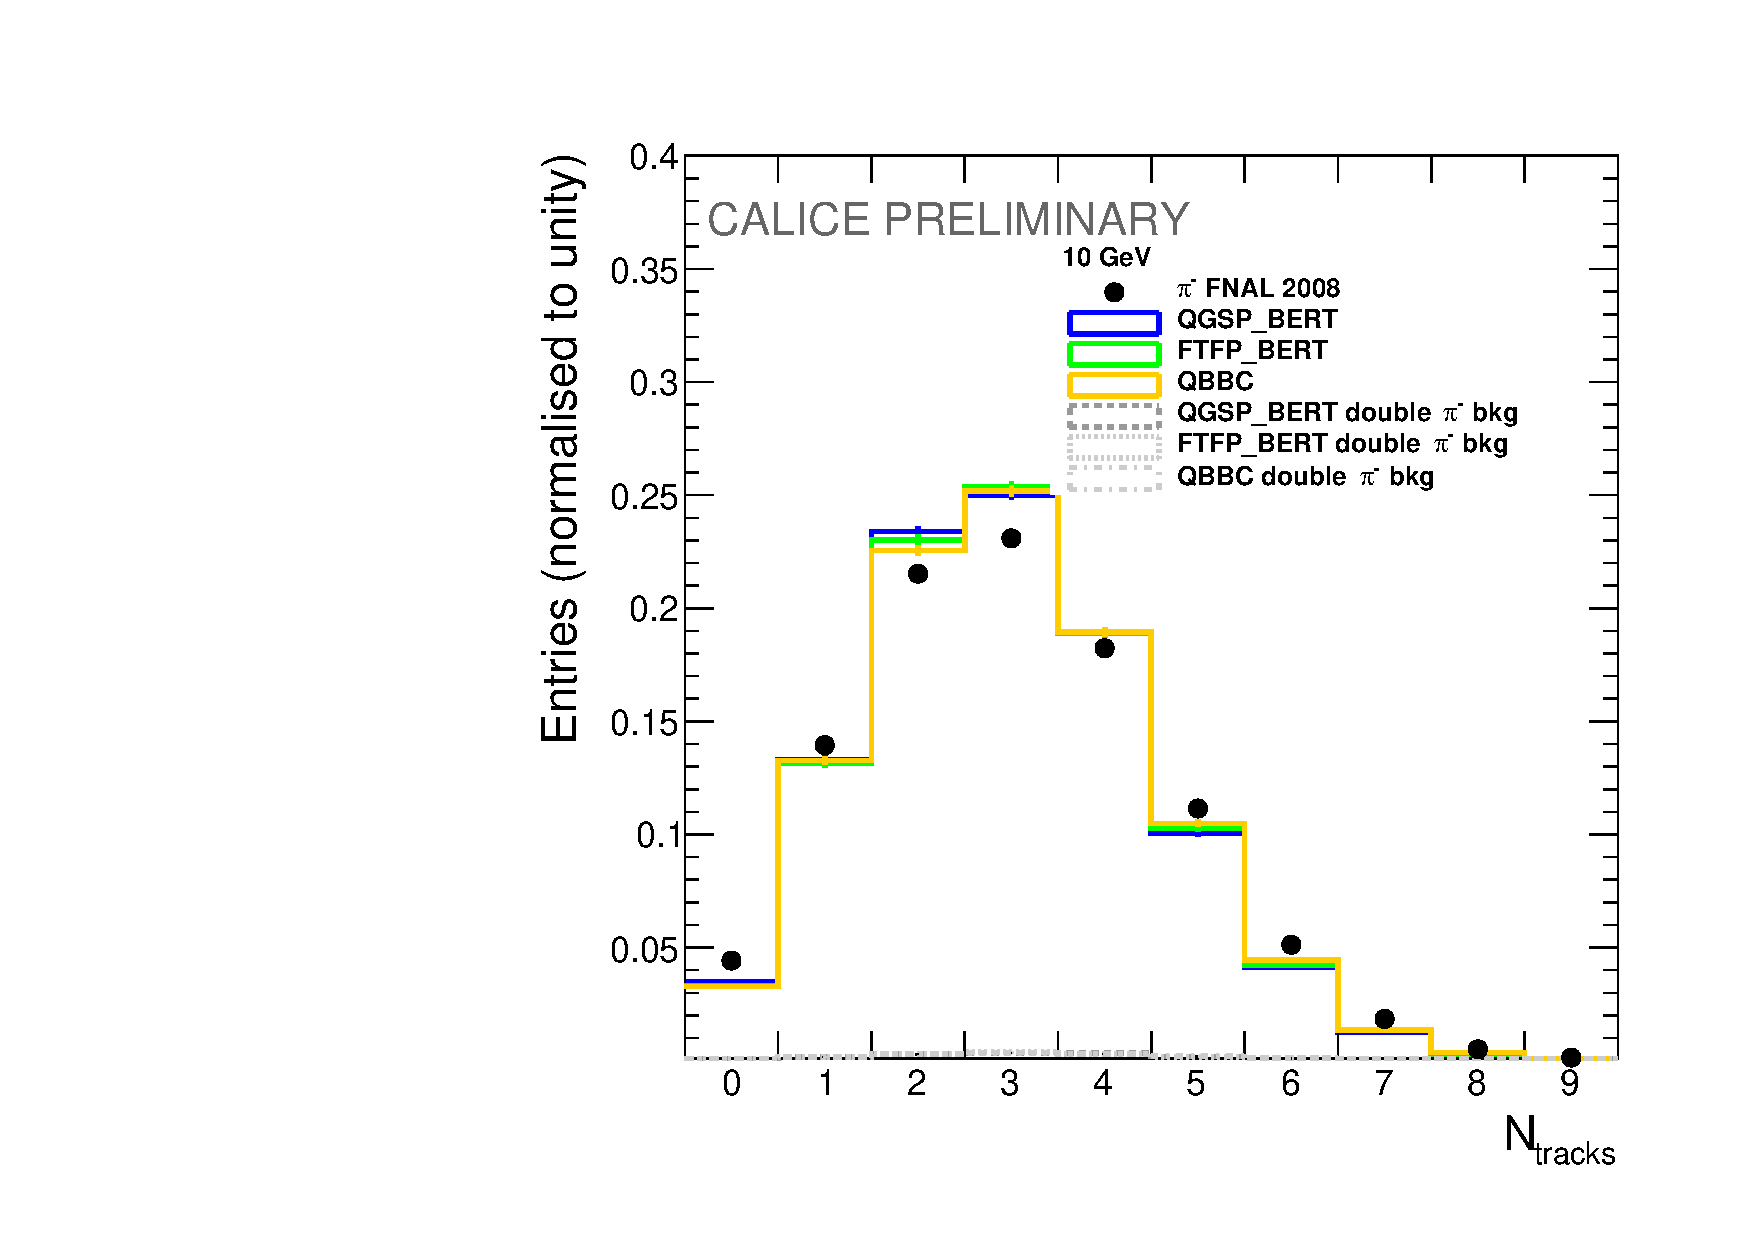
\includegraphics[width=.90\linewidth]{ECAL/plots/ntracks-10.pdf}
		\caption{\label{fig:tr10F} }
	\end{subfigure}
	\caption{\label{fig:trackexampleF} \sl Comparison of the number of secondary tracks between data Monte Carlo simulations for three {\sc Geant}4 physics lists  for energies of the primary particle of 2 (a) and 10 (b) GeV. Events without a detected interaction region according to Sec.~\ref{sec:iazone} are discarded. Error bars represent statistical errors only.}
\end{figure}

\begin{figure}
	\centering
	\begin{subfigure}{0.5\textwidth}
		\centering
		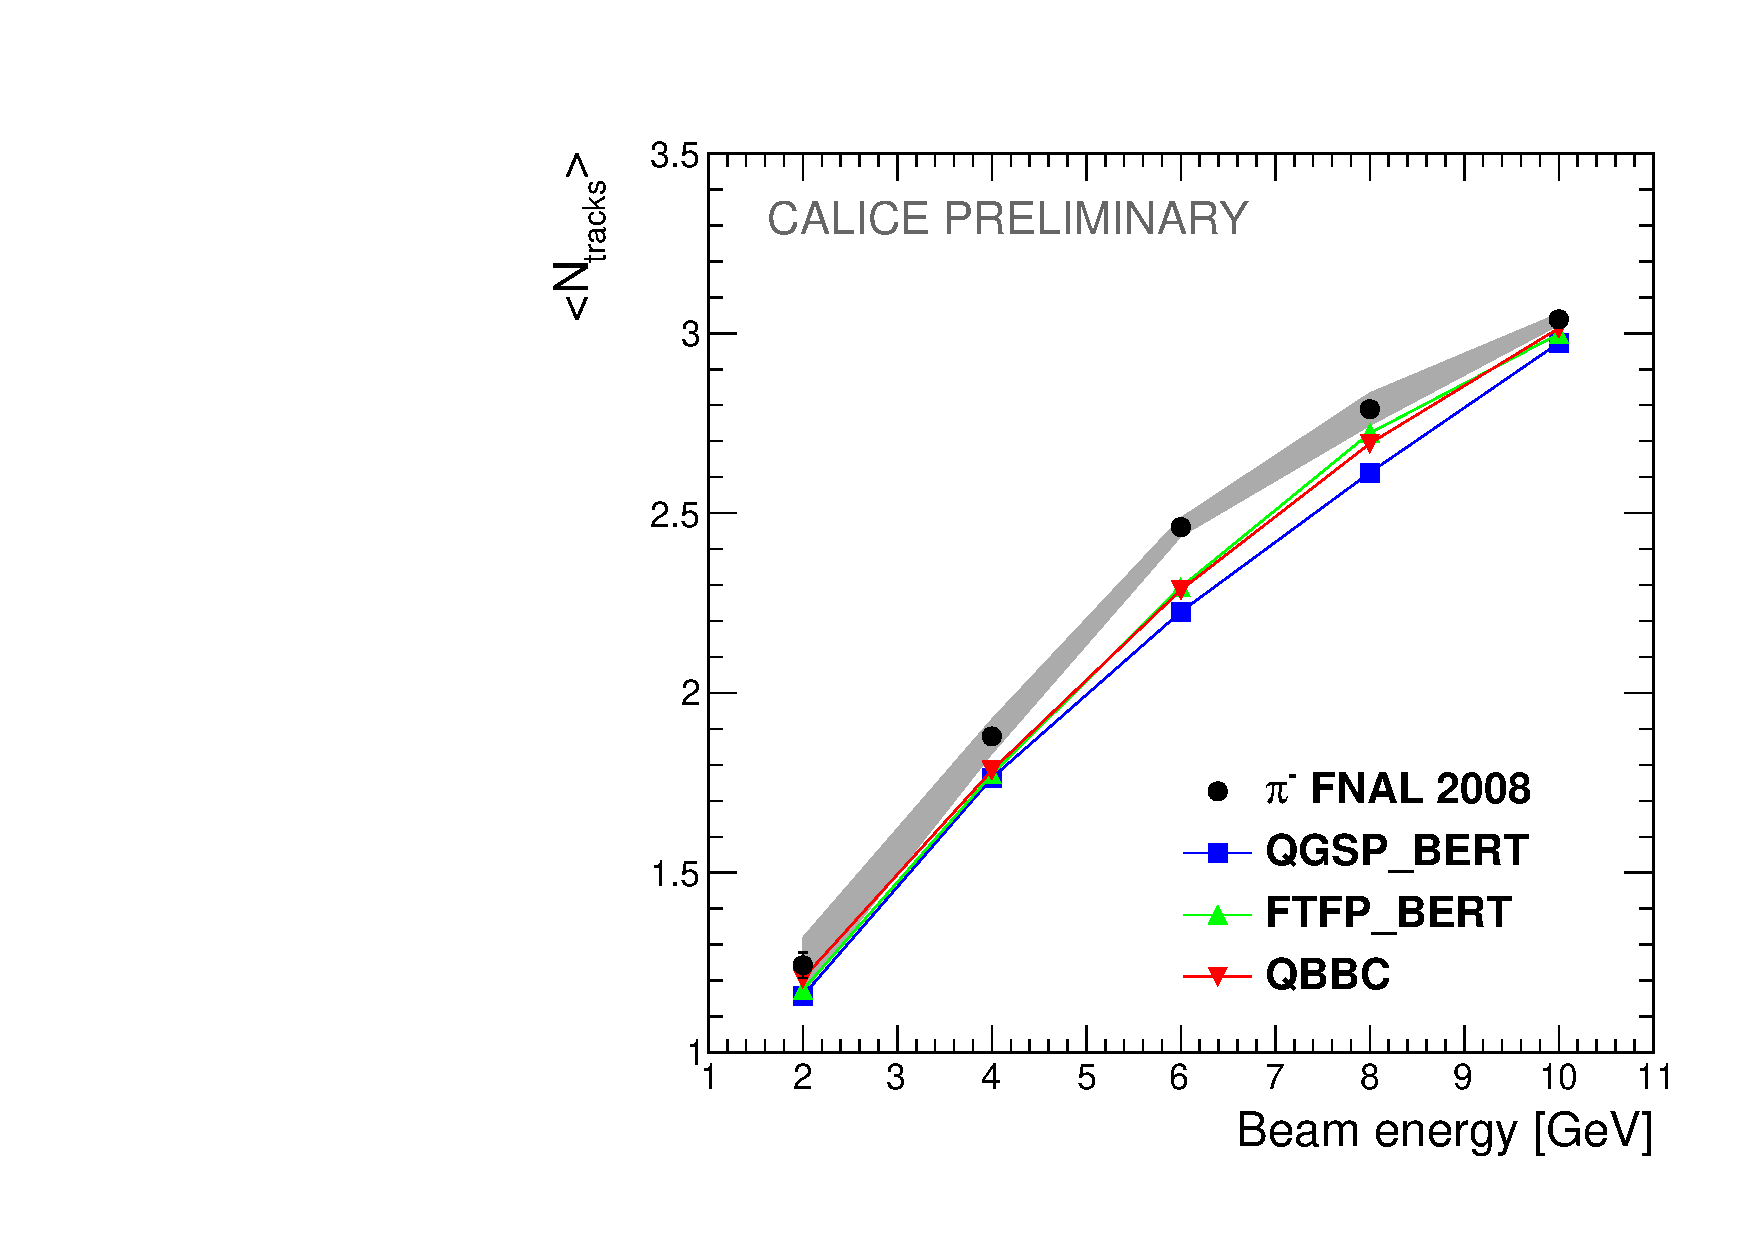
\includegraphics[width=.90\linewidth]{ECAL/plots/ntracks-graph.pdf}
		\caption{\label{fig:tracksgraphF} }
	\end{subfigure}% 
	\begin{subfigure}{0.5\textwidth}
		\centering
		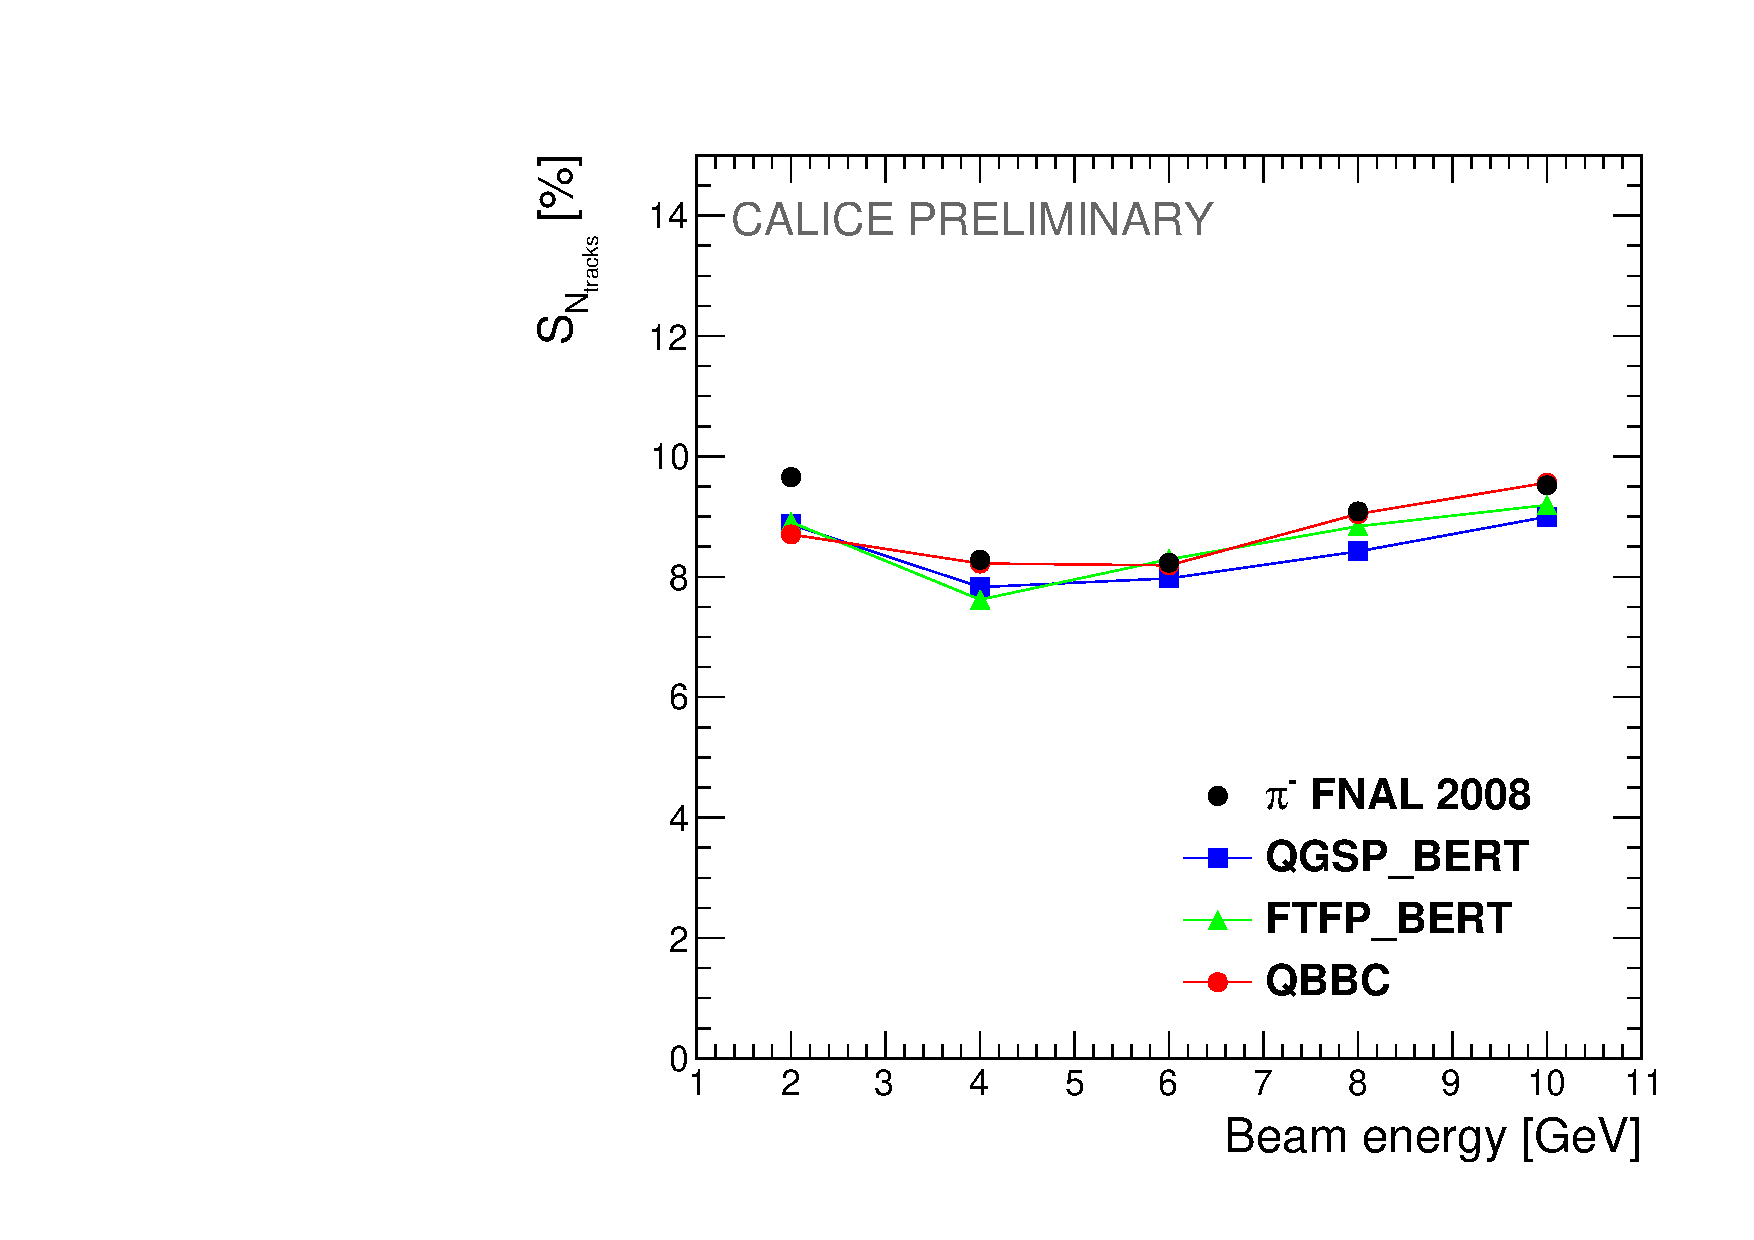
\includegraphics[width=.90\linewidth]{ECAL/plots/ntracks-graph-delta.pdf}
		\caption{\label{fig:dtracksgraphF}}
	\end{subfigure}
	\caption{\label{fig:fulltrackgraphF} \sl Mean number of secondary tracks $\left<N_{tracks}\right>$ for $\varepsilon = 0.03$ (a) and the corresponding sensitivity according to Eq.~\ref{eq:sens} of $\left<N_{tracks}\right>$ on the \ep\,(b) for data and Monte Carlo simulations for three {\sc Geant}4 physics lists as a function of the beam energy (from 2 to 10\,GeV). }
\end{figure}

\begin{figure}
	\centering
	\begin{subfigure}{0.5\textwidth}
		\centering
		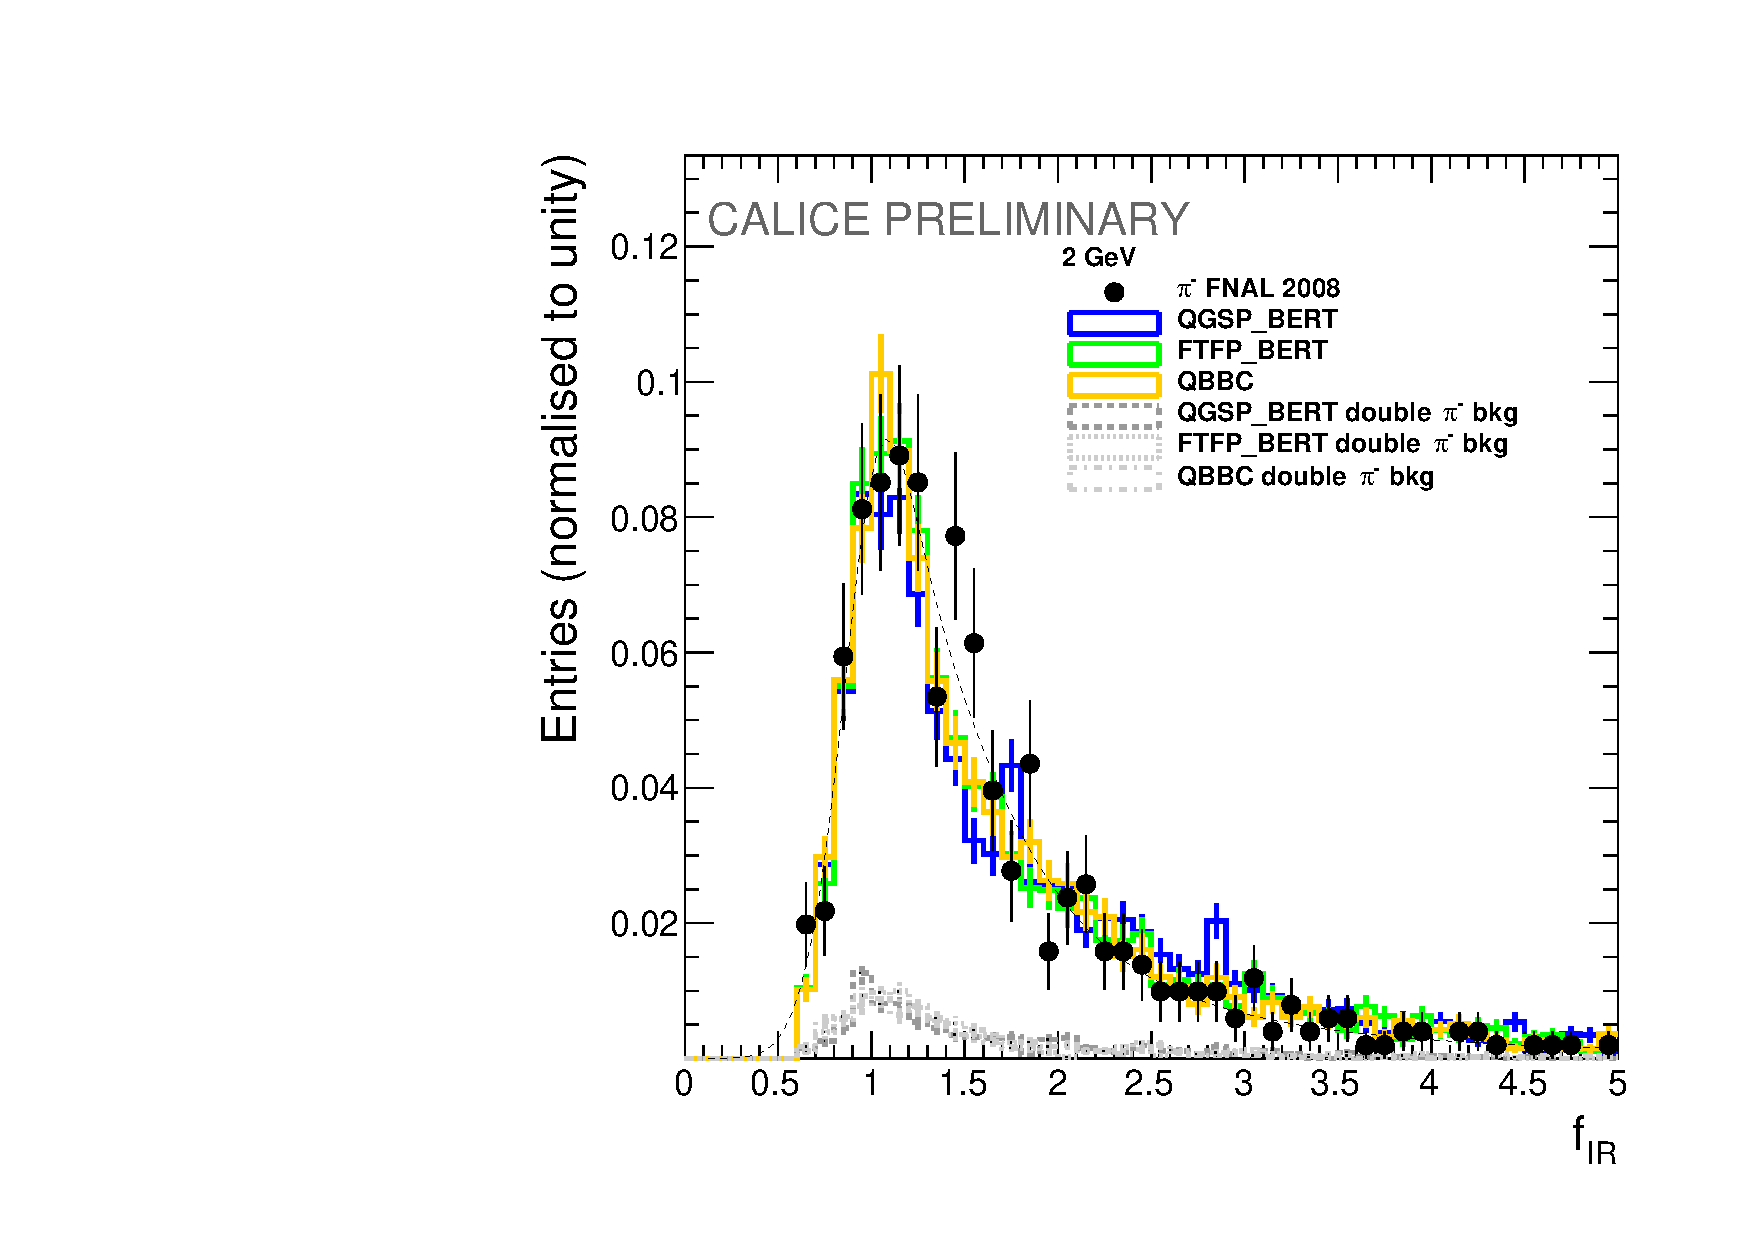
\includegraphics[width=.90\linewidth]{ECAL/plots/calibrationfit-2.pdf}
		\caption{\label{fig:calib2F} }
	\end{subfigure}% 
	\begin{subfigure}{0.5\textwidth}
		\centering
		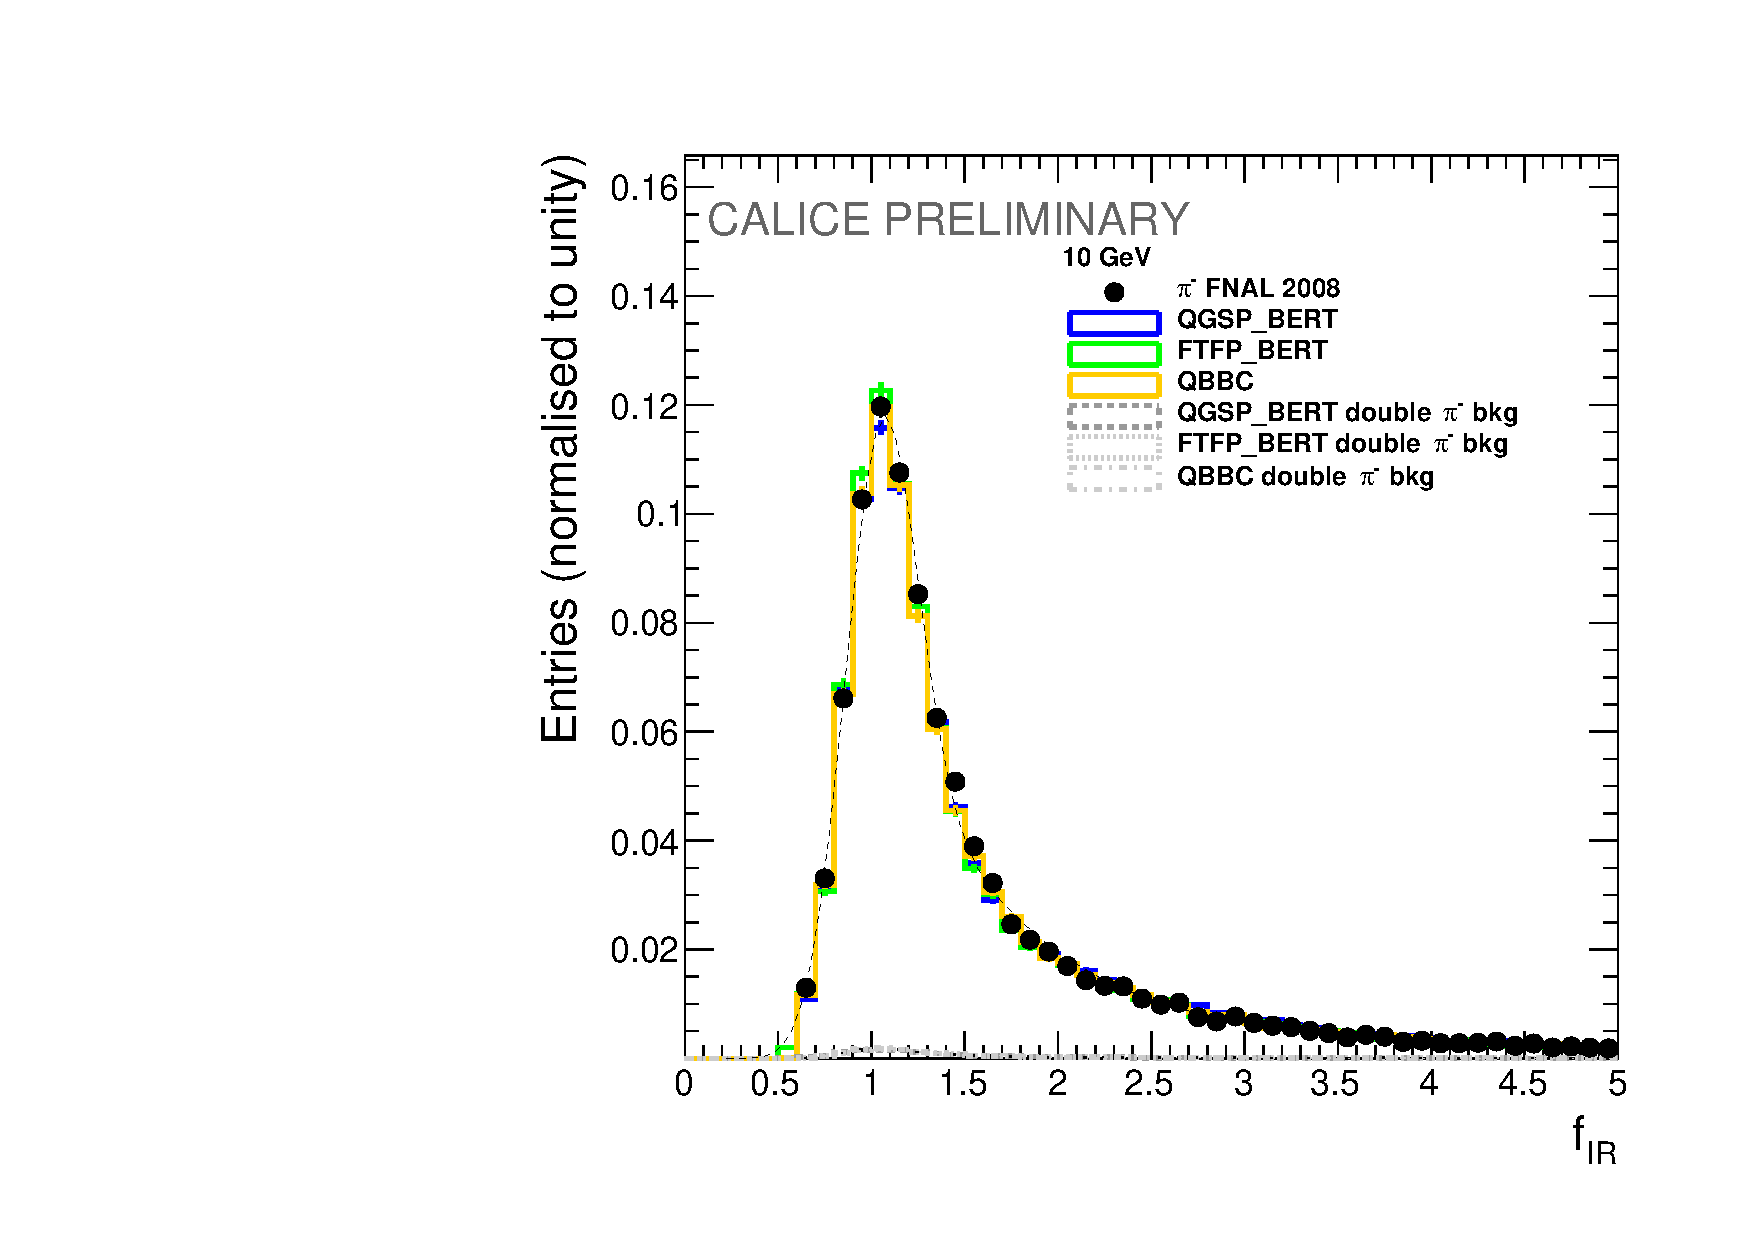
\includegraphics[width=.90\linewidth]{ECAL/plots/calibrationfit-10.pdf}
		\caption{\label{fig:calib10F} }
	\end{subfigure}
	\caption{\label{fig:calibF} \sl Histograms of the energy deposition in secondary tracks for the data with 2 (a) and 10 (b) GeV beam energies. The spectra are fitted by the convolution of a Landau and a Gaussian. Events without a detected interaction region according to Sec.~\ref{sec:iazone} are discarded. Error bars represent statistical uncertainties only.}
\end{figure}

\begin{figure}
	\centering
	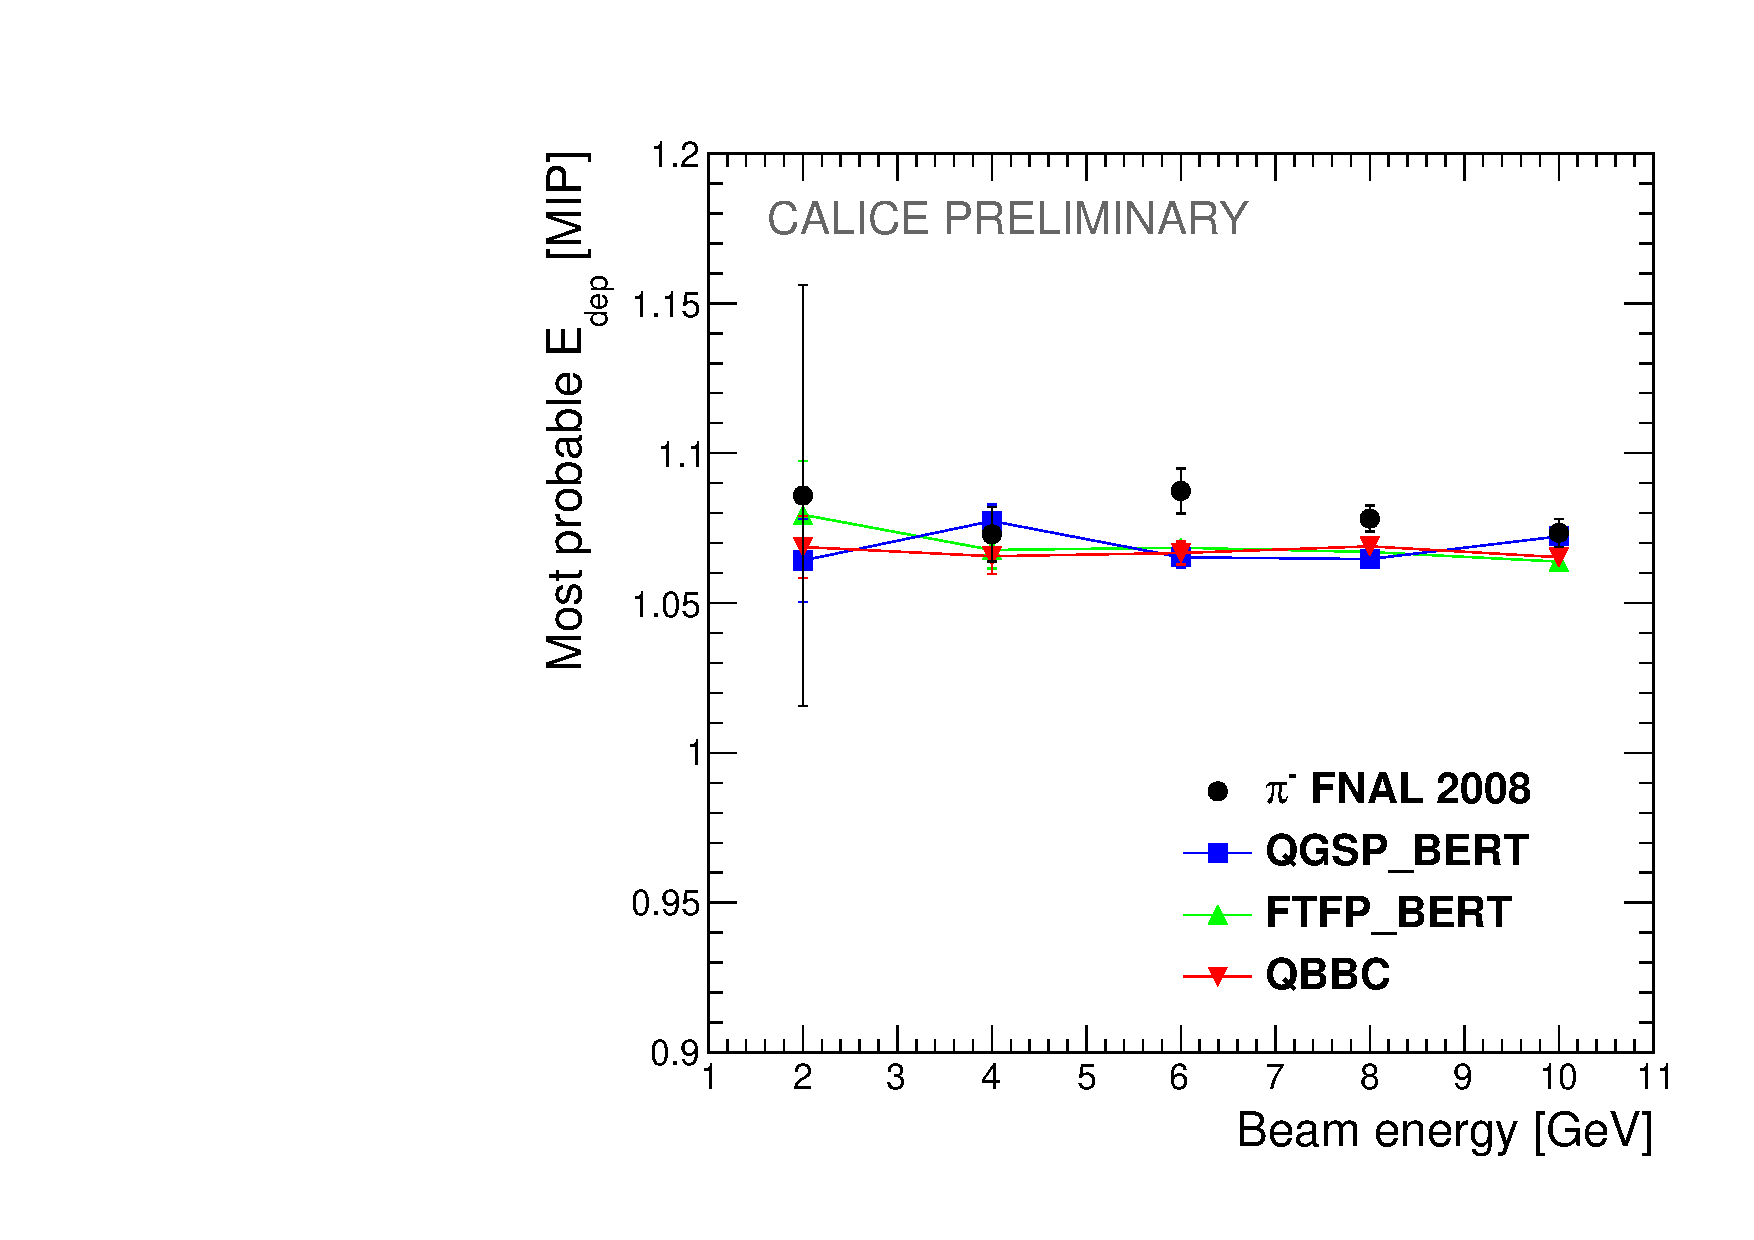
\includegraphics[width=0.5\textwidth]{ECAL/plots/calibrationfit-graph.pdf}
	\caption{\label{fig:calibrationgraphF} \sl MPV of the Landau fit to the $E_{dep}^t$ distributions of the pencil-like secondary tracks as a function of the beam energy for $\pi^-$ data and three Monte Carlo samples. The MPV point the of 2\,GeV data sample is excluded because of the small statistics left after selection. Events without a detected interaction region  according to Sec.~\ref{sec:iazone} are discarded.  Error bars represent the statistical fit uncertainty.}
\end{figure}

%-----------------------------------------------------------------------------
%-----------------------------------------------------------------------------
%-----------------------------------------------------------------------------

\subsection*{Les quarks top et bottom \'a l'ILC}
Electroweak production of the fermion pairs proceeds through the $f\bar{f}X$ vertex, where $X$ represents neutral vector bosons, photon or $Z^0$ boson.  The current at the $f\bar{f}X$ vertex can be expressed via form factors $F$ as 
\begin{equation}
\Gamma^{f\bar{f}X}_\mu (k^2,q,\bar{q}) = ie\{ \gamma_\mu (F^X_{1V}(k^2) + \gamma^5 F^X_{1A}(k^2)) - \frac{\sigma_{\mu\nu}(q-\bar{q})^\nu}{2m_f}(iF^X_{2V}(k^2) + \gamma^5 F^X_{2A}(k^2)) \},
\end{equation}
where $k^2= (q+\bar{q})^2$ is the four momentum squared of the exchanged vector boson, $q$ and $\bar{q}$ are the four vectors of the fermion $f$ and antifermion $\bar{f}$ and $m_f$ is the fermion mass. Further, $\gamma_\mu$ and $\gamma_5$ are the Dirac matrices, and $\sigma_{\mu\nu} = i/2(\gamma_\mu\gamma_\nu - \gamma_\nu\gamma_\mu)$.

The \sm\ values of the form factors are the following:
\begin{equation}
F^{f\gamma}_{1V} = Q^{f}, \ F^{f\gamma}_{1A} = 0, \ F^{fZ}_{1V} = \frac{I^f - 2Q^f\sin^2\theta_W}{2\cos\theta_W\sin\theta_W}, \ F^{fZ}_{1A} = - \frac{I^f}{2\cos\theta_W\sin\theta_W},
\label{formula:SMformFactors_3F}
\end{equation}
and all $F_2$ factor are zero. In the Eq.~\ref{formula:SMformFactors_3F} $I^f$ is the weak isospin number, $I^t = 1/2$ for top and $I^b = -1/2$ for bottom quark and $Q^f$ is the electric charge, $Q^t = 2/3$ and $Q^b = -1/3$.

%The form factors are related to fermion couplings with left and right-handed helicity to $Z^0$ boson:
The following definition of the left-handed and right handed $Z^0b\bar{b}$ couplings is used throughout the thesis: 
\begin{equation}
%g_L^Z = (F_{1V}^Z - F_{1A}^Z), \  g_R^Z = F_{1V}^Z + F_{1A}^Z, 
g_L^Z = I^f - Q^f\sin^2\theta_W, \  g_R^Z = -Q^f\sin^2\theta_W, 
\label{formula:EWcouplings_3F}
\end{equation}

%-----------------------------------------------------------------------------
%-----------------------------------------------------------------------------
%-----------------------------------------------------------------------------

\subsection*{Reconstruction de la charge du quark bottom}

\begin{figure}
	{\centering
		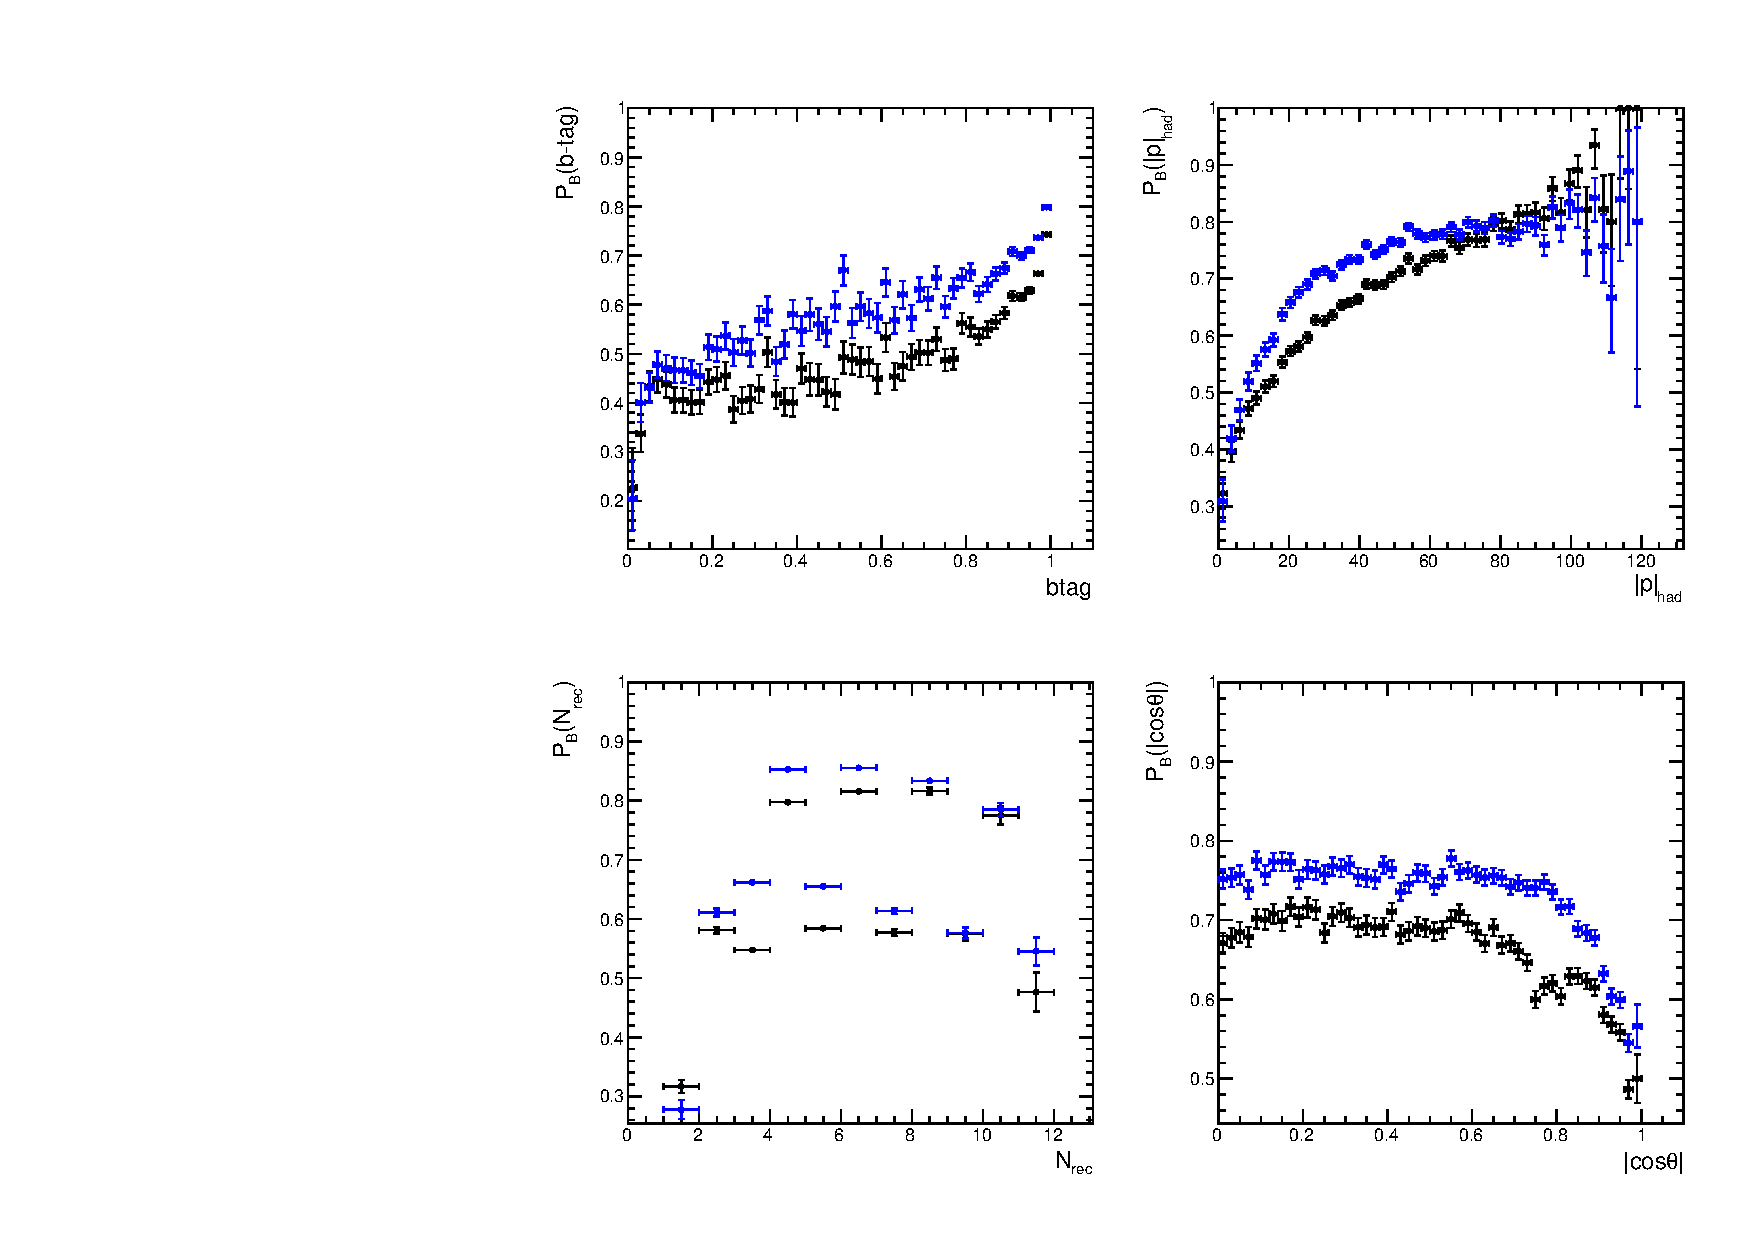
\includegraphics[width=0.95\textwidth]{ILD/plots/recovery-purity-comparison.pdf}
		\caption{\sl Comparison of the purity as function of the jet b-tag, reconstructed b-hadron momentum, $N_{rec}$ and the polar angle $|\cos\theta|$ before and after the vertex recovery algorithm.  
		}
		\label{fig:RecoveryPurityComparison_3F}
	}
\end{figure}

\begin{figure}
	{\centering
		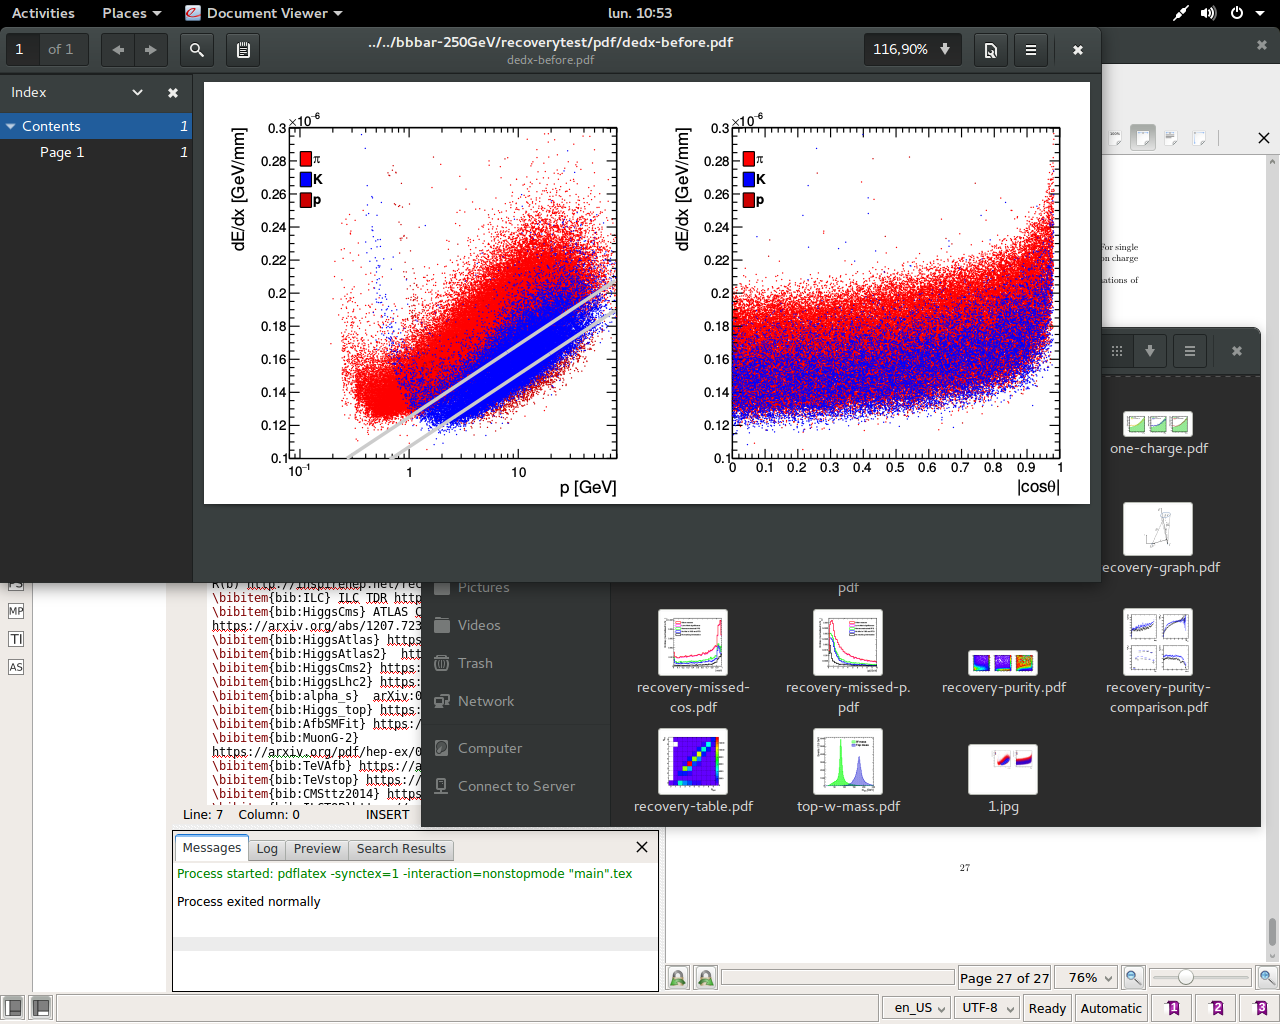
\includegraphics[clip, trim=8cm 18.5cm 7cm 4cm,width=0.95\textwidth]{ILD/plots/dedx-before.png}
		\caption{\sl The energy deposition per track length $dE/dx$ as function of the particle momentum, the particle polar angle $|\cos\theta|$ for different particles. Two gray lines separate out the region with a maximal kaon concentration. 
		}
		\label{fig:dEdxBefore_3F}
	}
\end{figure}

\begin{figure}
	{\centering
		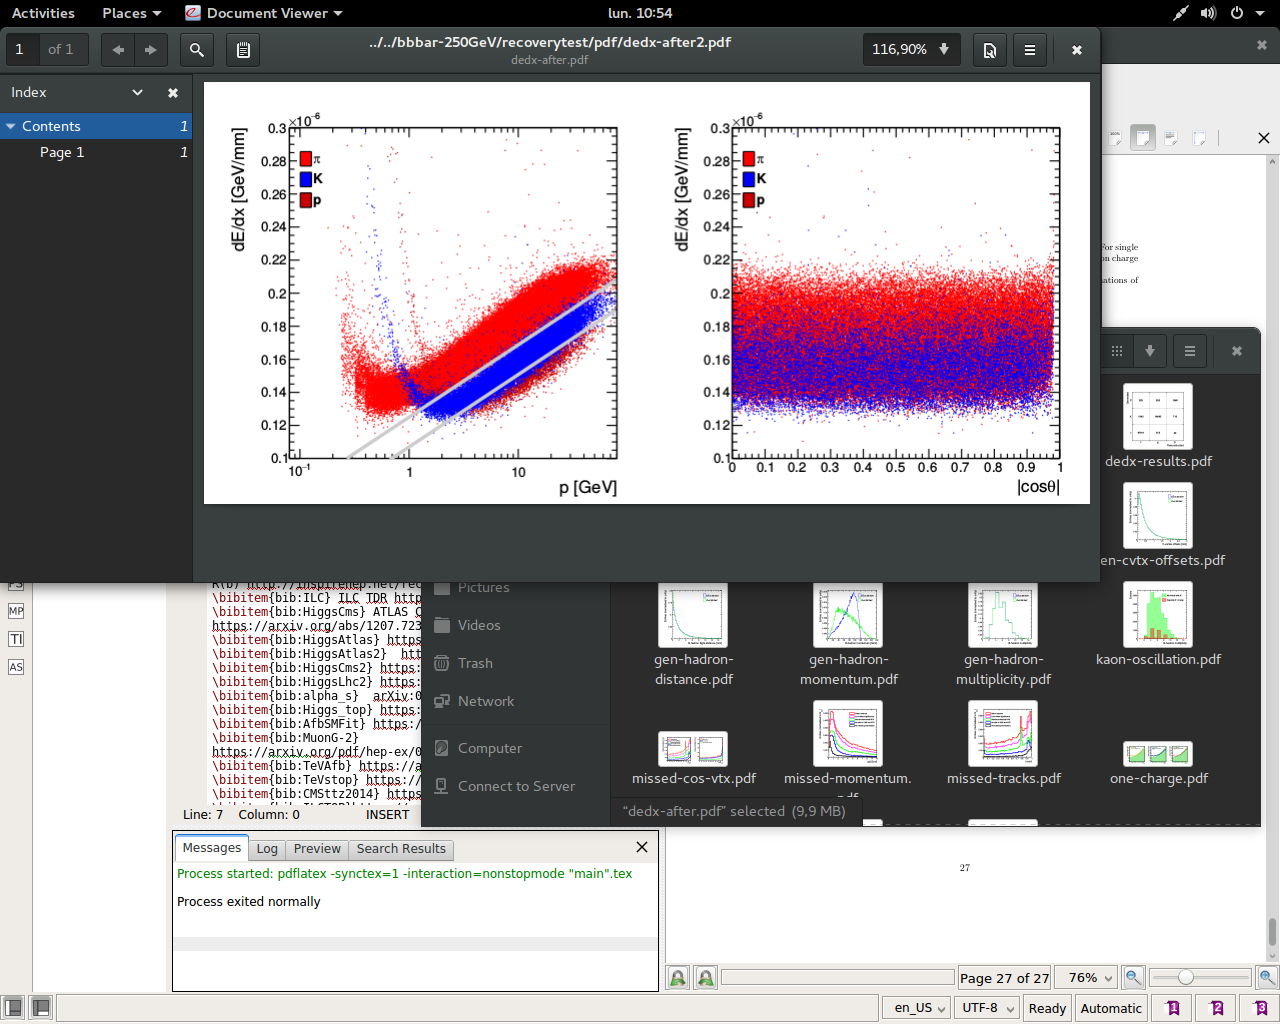
\includegraphics[clip, trim=8cm 18.5cm 7cm 4cm, width=0.95\textwidth]{ILD/plots/dedx-after.png}
		\caption{\sl The energy deposition per track length $dE/dx$ as function of the particle momentum, the particle polar angle $|\cos\theta|$ for different particles after application of the angular correction, described in text. Two gray lines separate out the region with a maximal kaon concentration. 
		}
		\label{fig:dEdxAfter_3F}
	}
\end{figure}


%-----------------------------------------------------------------------------
%-----------------------------------------------------------------------------
%-----------------------------------------------------------------------------

\subsection*{Reconstruction de l'angle polaire du quark top}


\begin{figure}
	\centering
	\begin{subfigure}{0.5\textwidth}
		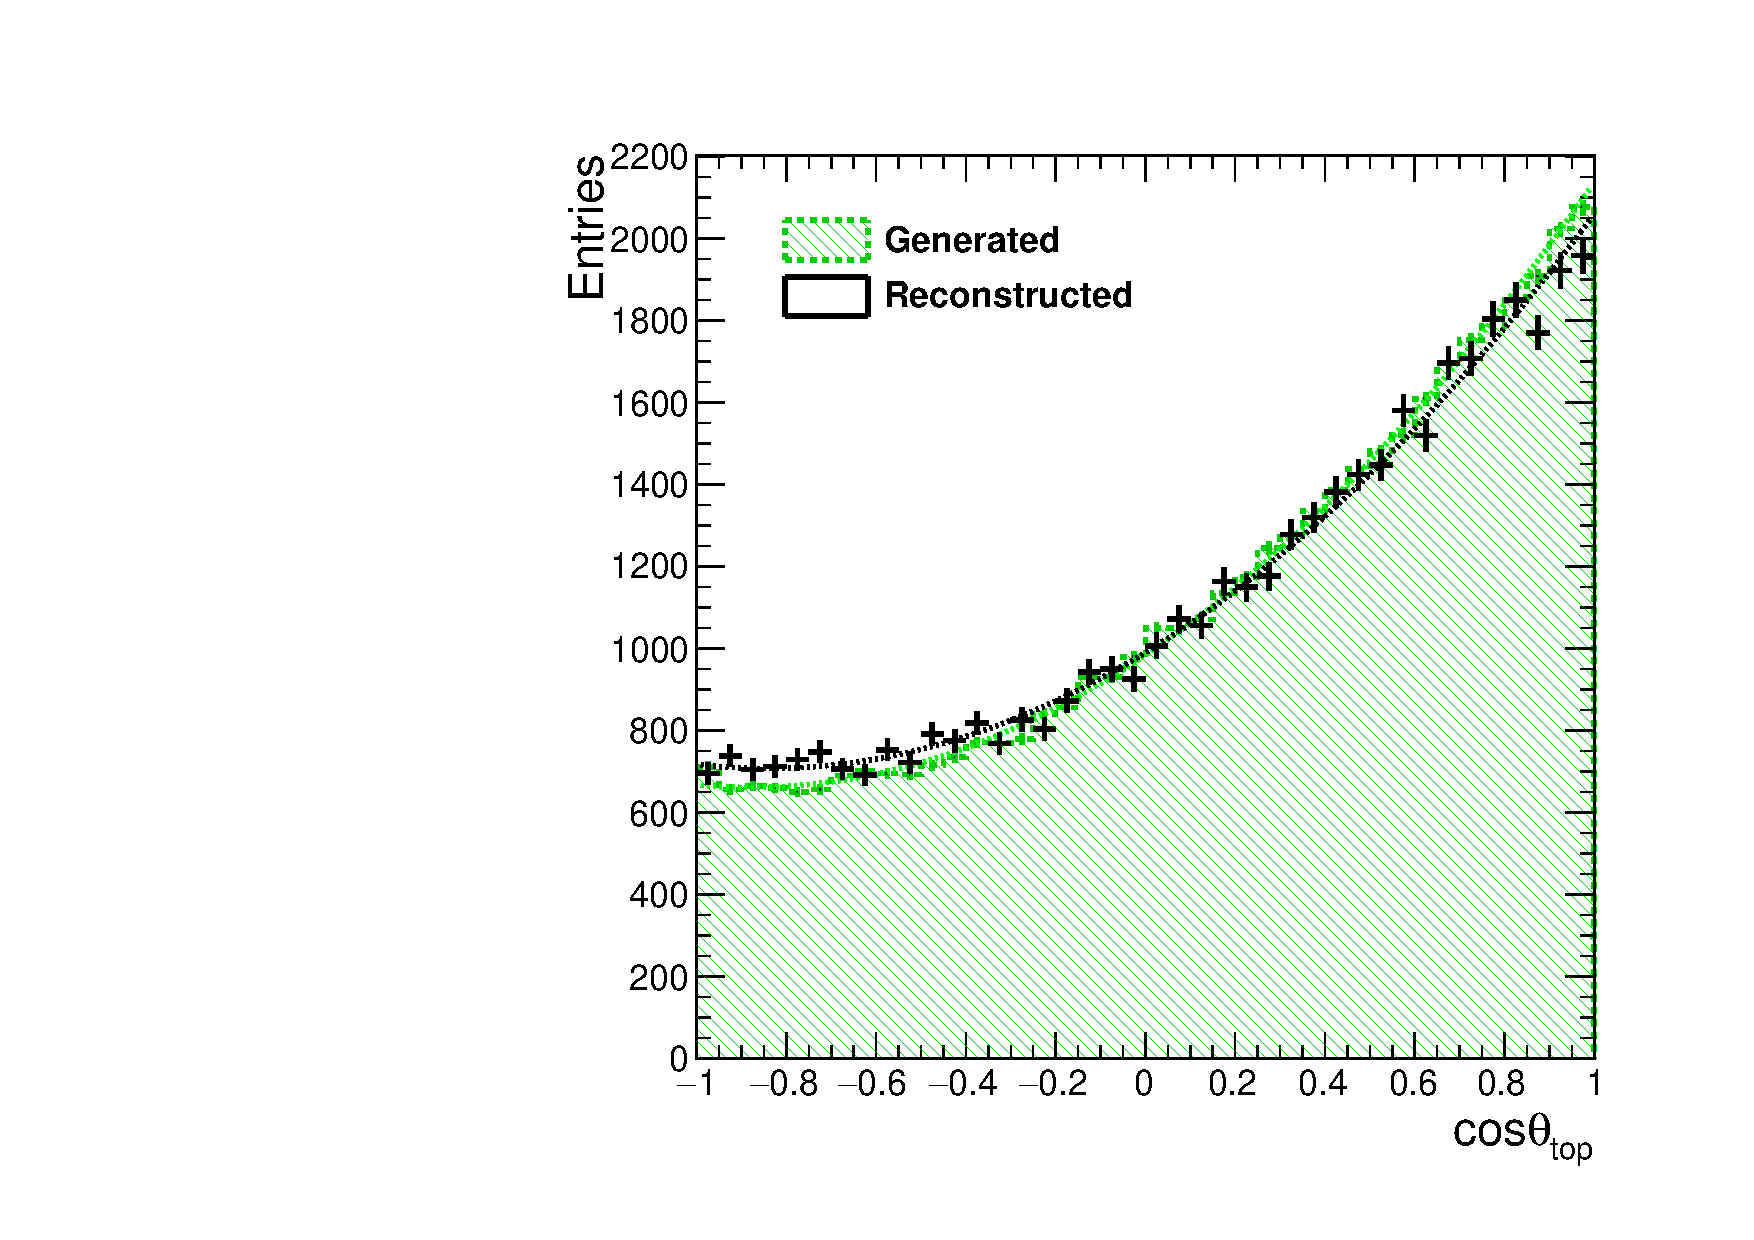
\includegraphics[width=0.95\textwidth]{ILD/plots/top-asymmetry-lepton.pdf}
		\caption{\label{fig:TopAsymmetryChi_a_3F} }
	\end{subfigure}% 
	\begin{subfigure}{0.5\textwidth}
		\centering
		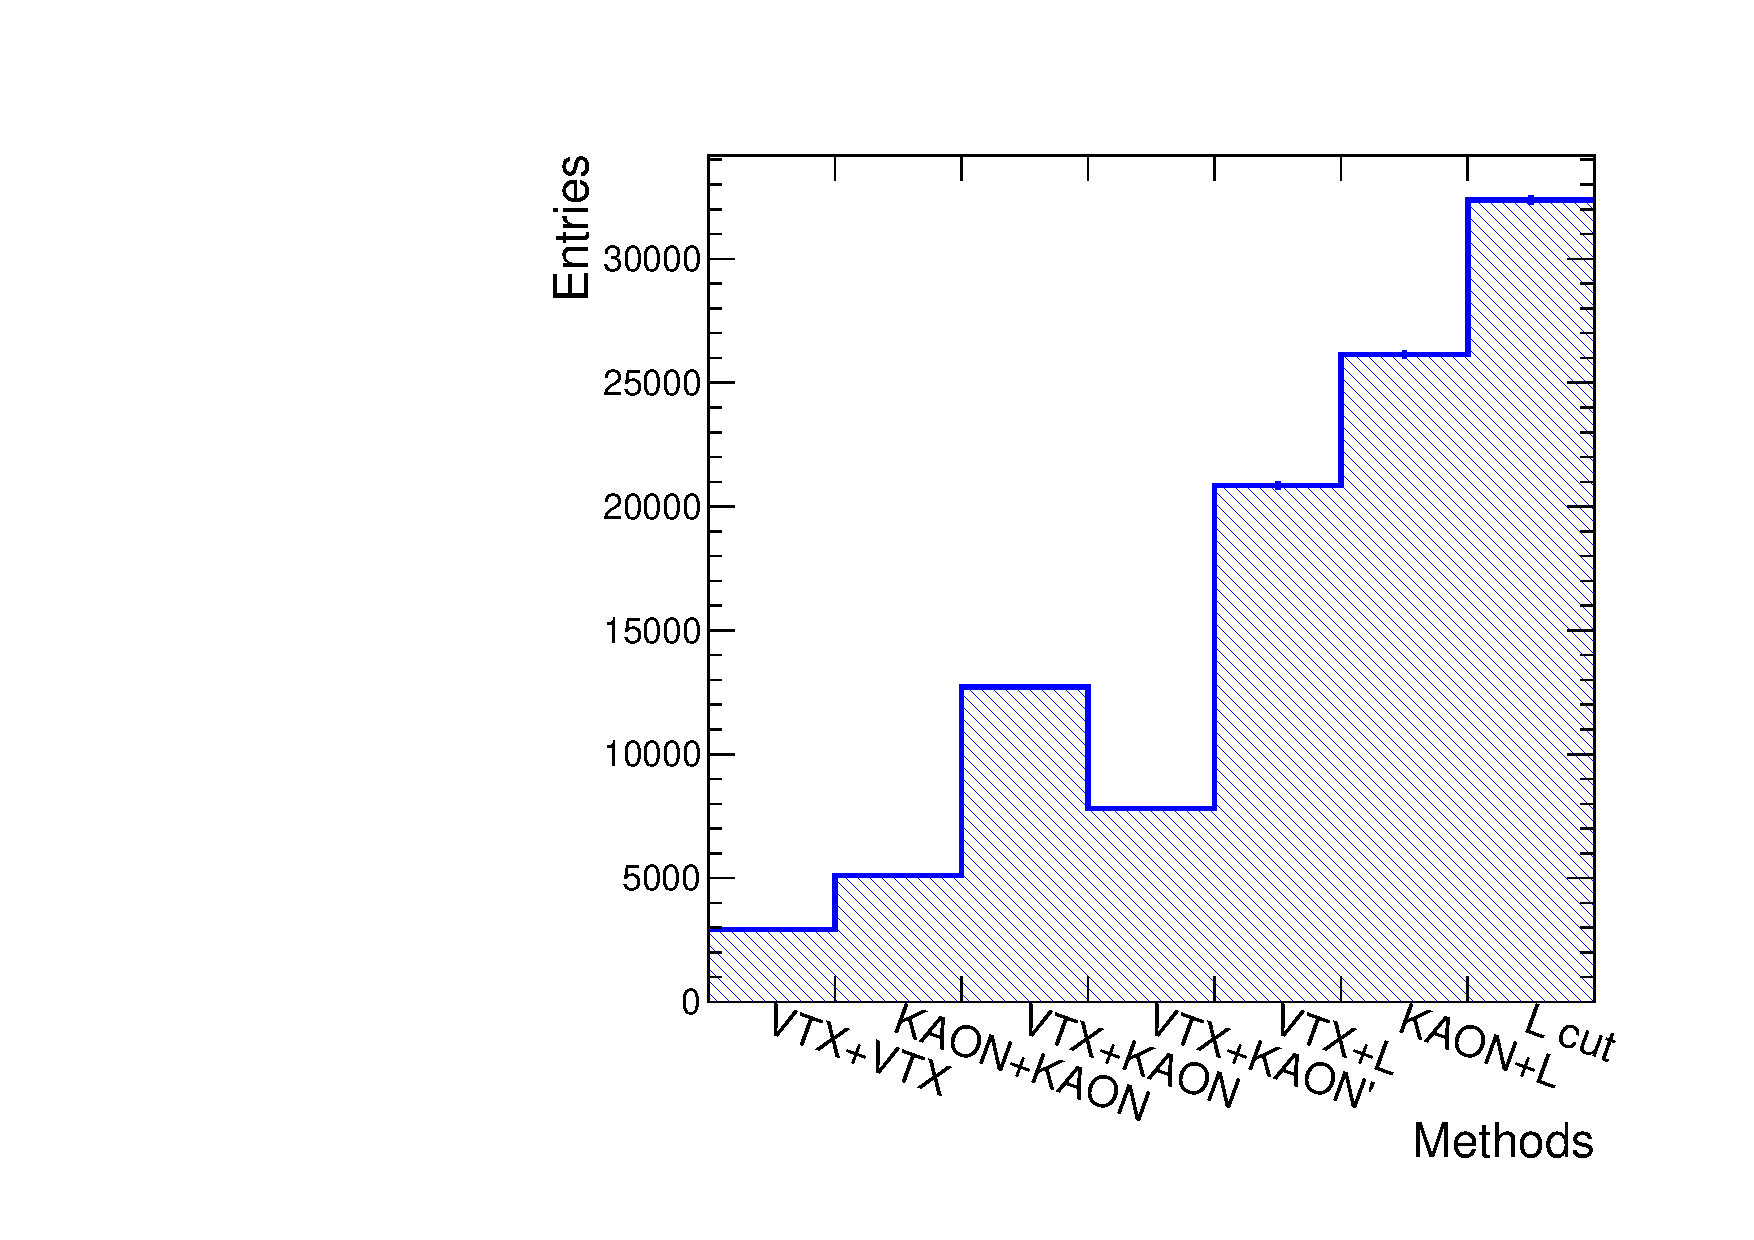
\includegraphics[width=0.95\textwidth]{ILD/plots/top-methods-lepton.pdf}
		\caption{\label{fig:TopAsymmetryChi_b_3F} }
	\end{subfigure}
	\caption{\sl Generated polar angle distribution compared to reconstructed polar angle (a) using all possible charge signature combinations, plotted in (b). }
	\label{fig:TopAsymmetryChi_3F}
\end{figure}

%-----------------------------------------------------------------------------
%-----------------------------------------------------------------------------
%-----------------------------------------------------------------------------

\subsection*{Reconstruction de l'angle polaire du quark bottom}

\begin{figure}
	\centering
	\begin{subfigure}{0.5\textwidth}
		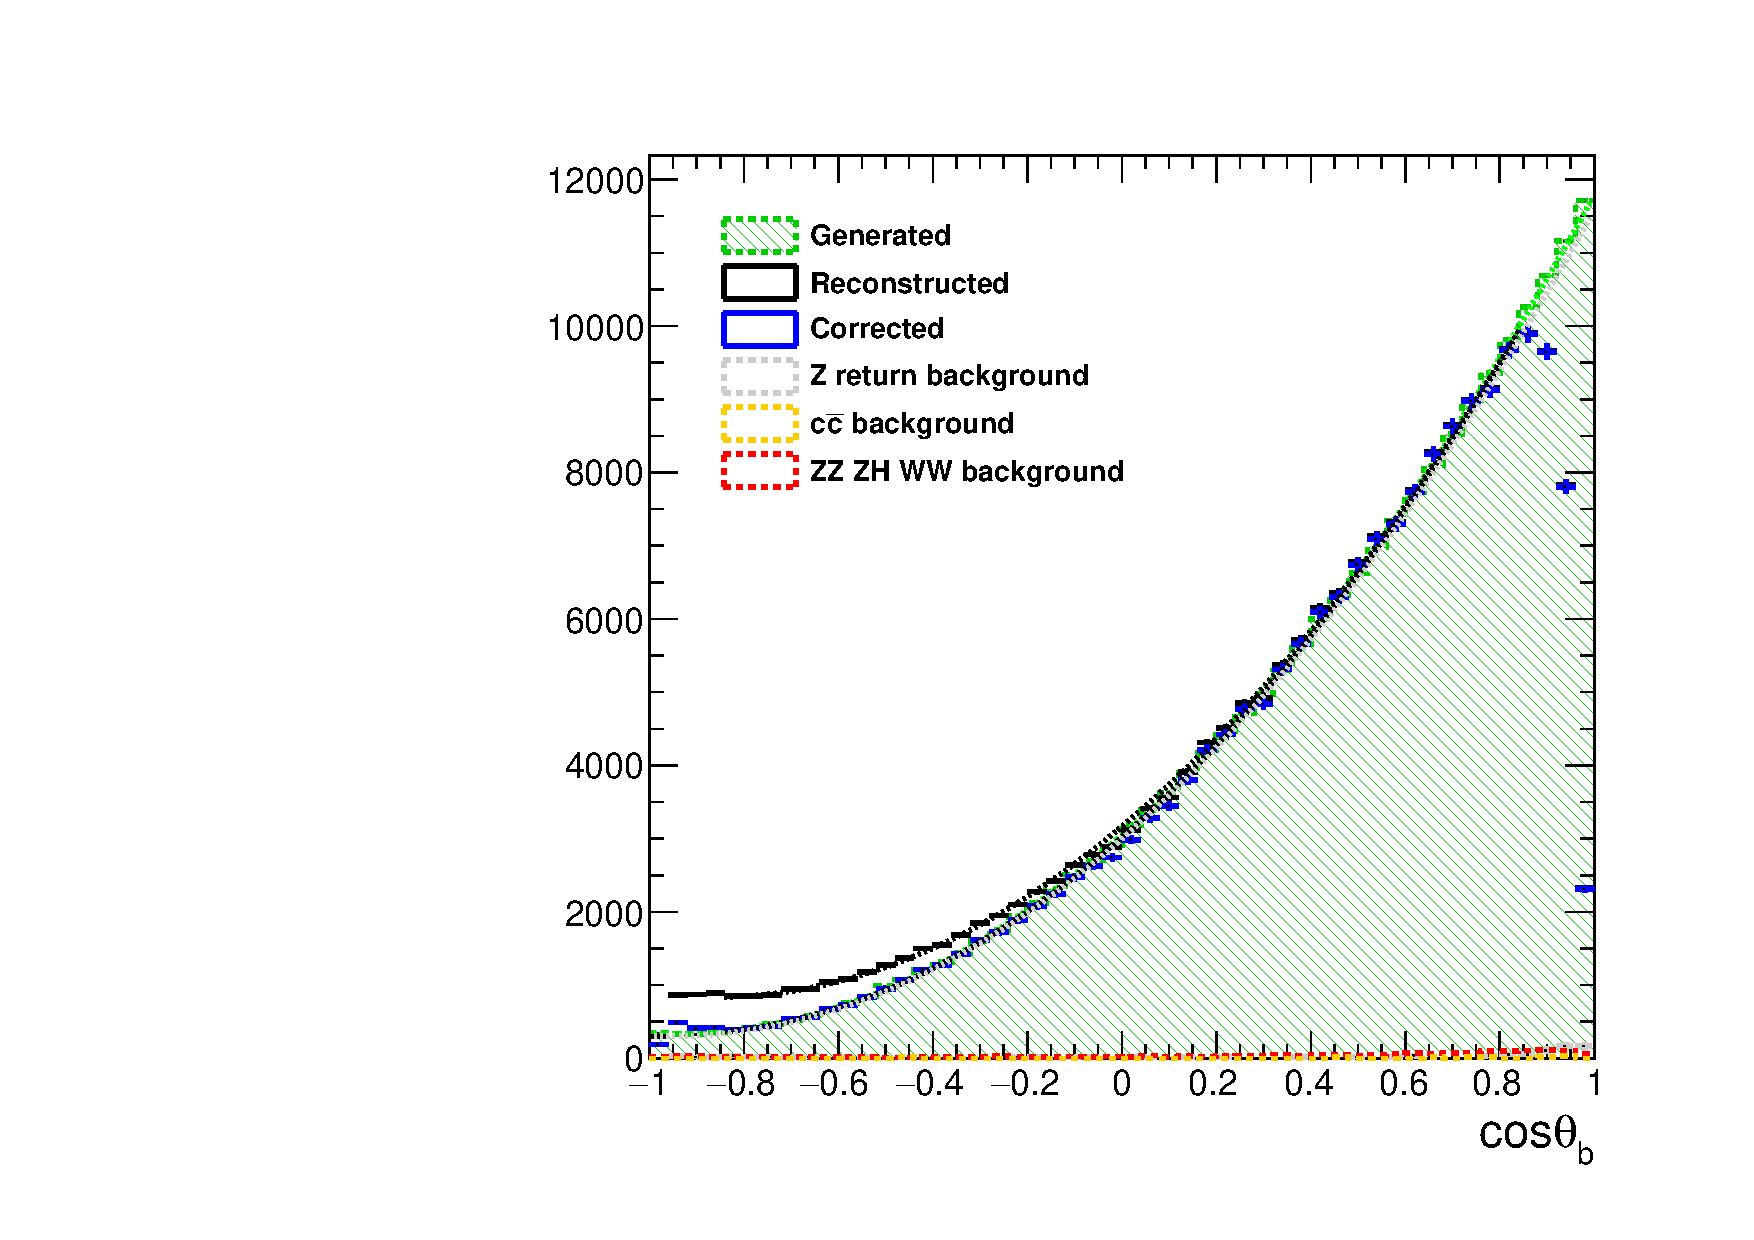
\includegraphics[width=0.95\textwidth]{ILD/plots/basymmetry-final-left.pdf}
		\llap{\shortstack{%
				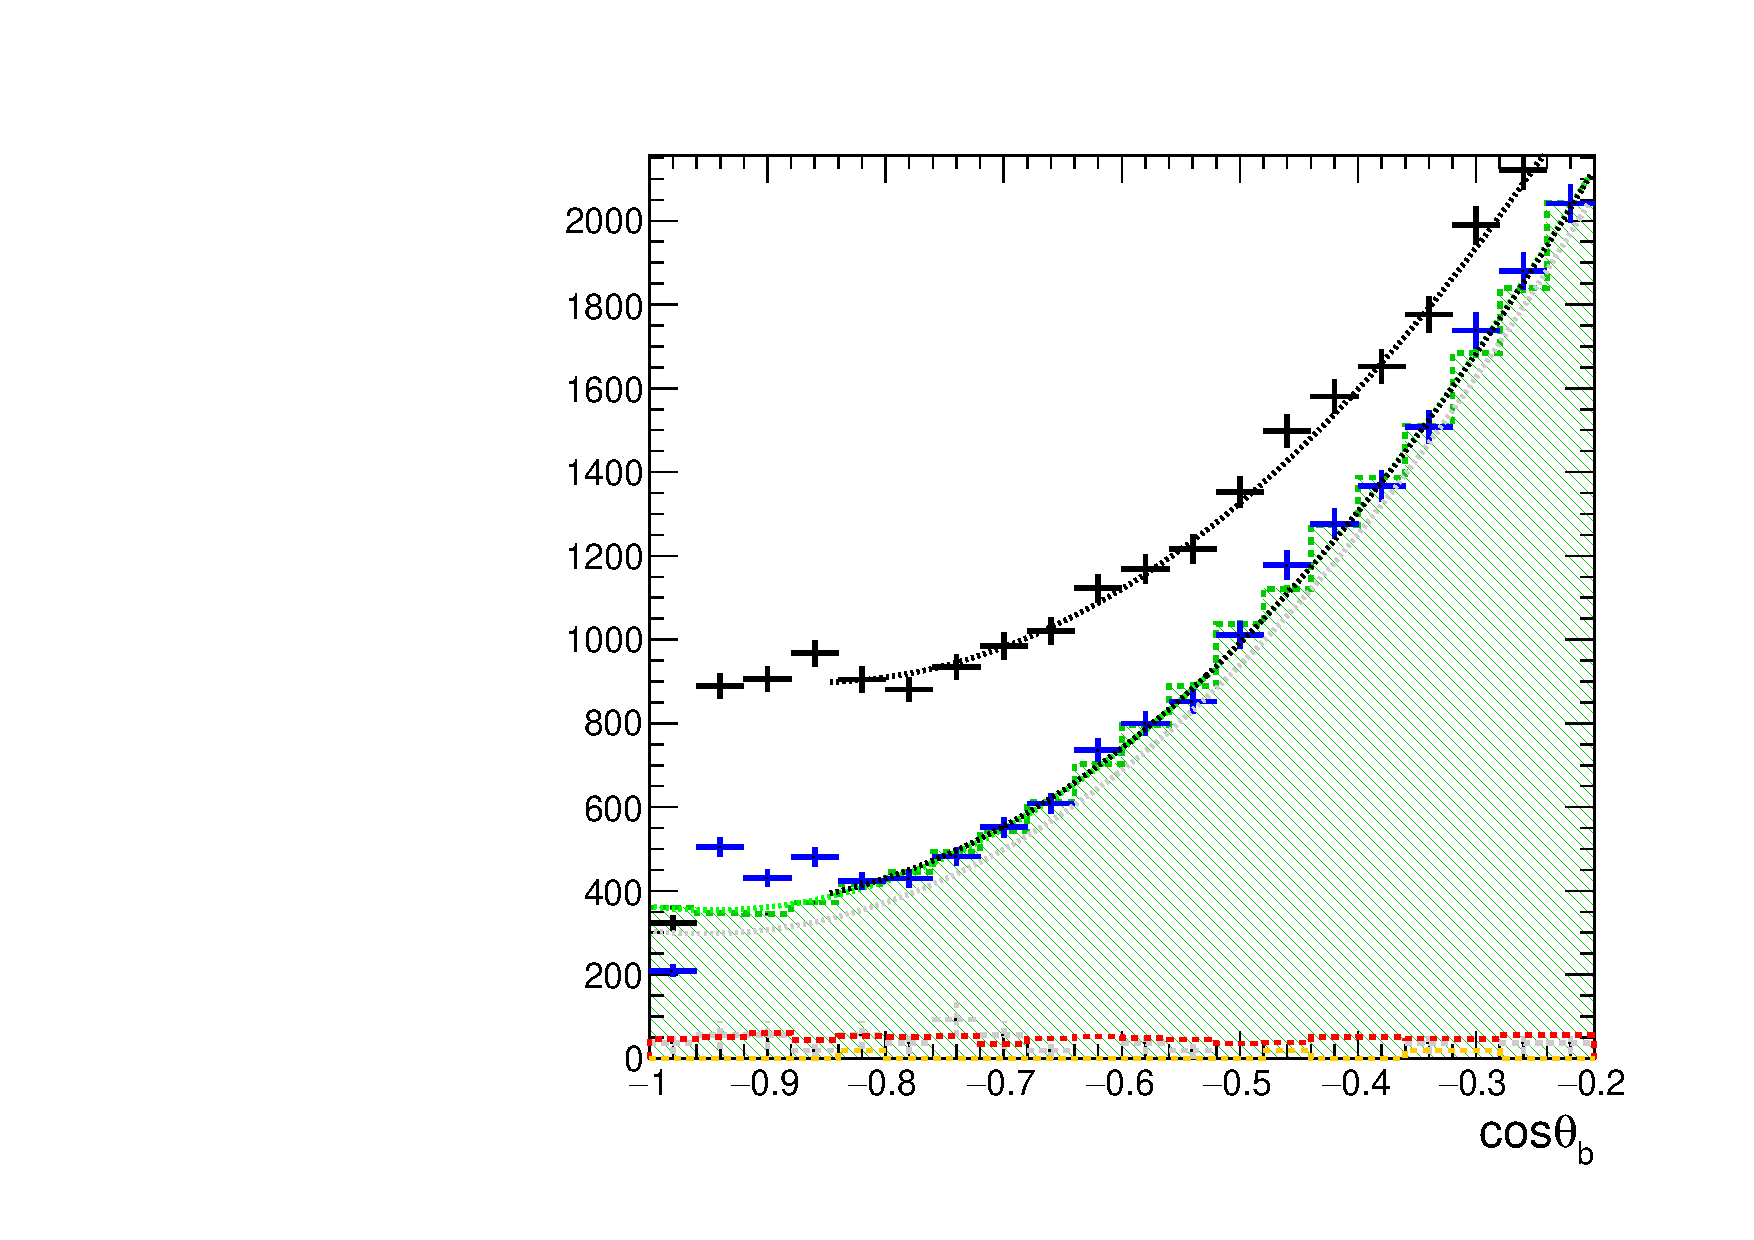
\includegraphics[clip, trim=0cm 0cm 1.8cm 1.7cm, scale=.14]{ILD/plots/zoom-final.pdf}\\
				\rule{0ex}{0.38in}%
			}
			\rule{1.8in}{0ex}}
		\caption{\label{fig:BAsymmetryFinal_a_3F} }
	\end{subfigure}% 
	\begin{subfigure}{0.5\textwidth}
		\centering
		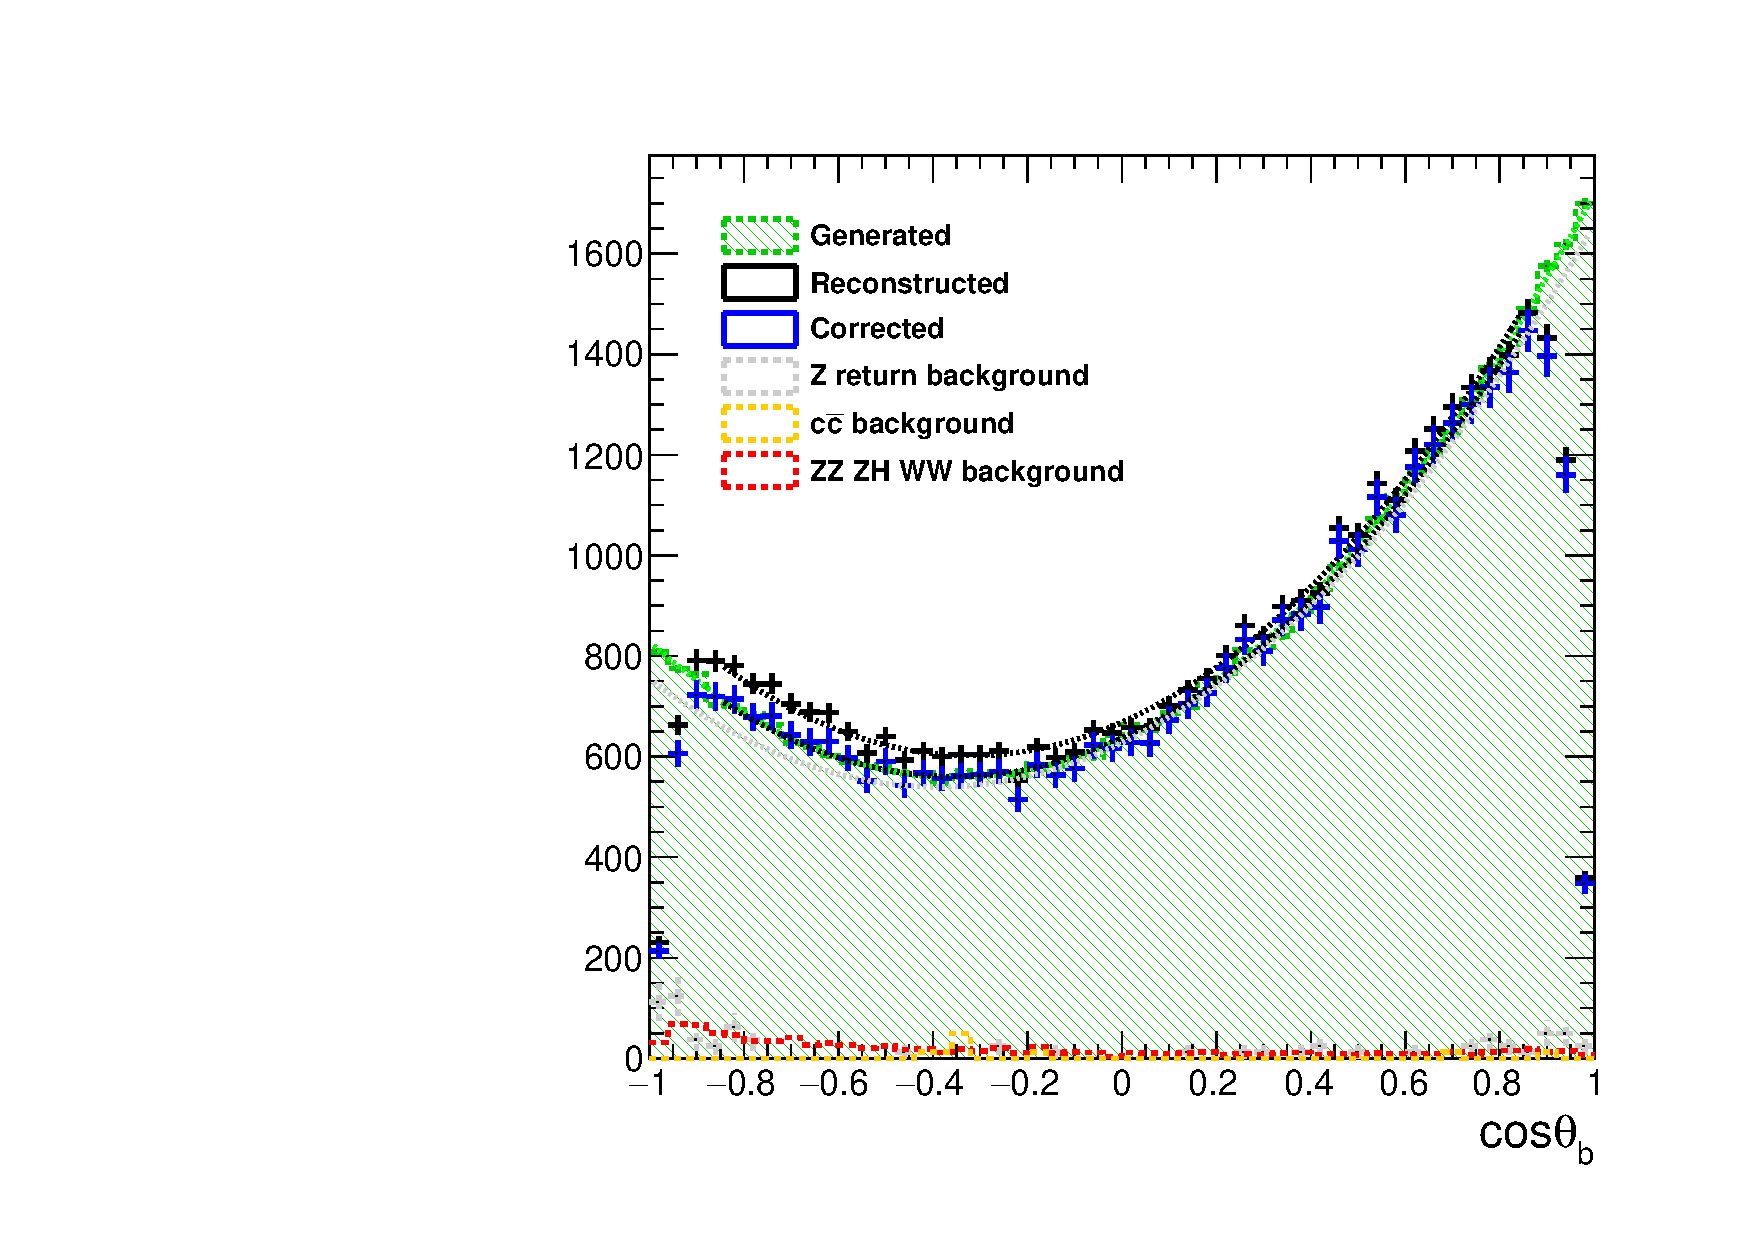
\includegraphics[width=0.95\textwidth]{ILD/plots/basymmetry-final-right.pdf}
		\caption{\label{fig:BAsymmetryFinal_b_3F} }
	\end{subfigure}
	\caption{\sl Generated b-quark polar angle distribution compared to the final reconstructed b-quarks polar angle in left-handed case (a) and right-handed case (b) with overlaid background processes.  }
	\label{fig:BAsymmetryFinal_3F}
\end{figure}



\begin{figure}
	\centering
	\begin{subfigure}{0.5\textwidth}
		\includegraphics[width=0.99\textwidth]{ILD/plots/lep-result-zoom.pdf}
		\caption{\label{fig:LEPILCResult_a_3F} }
	\end{subfigure}% 
	\begin{subfigure}{0.5\textwidth}
		\centering
		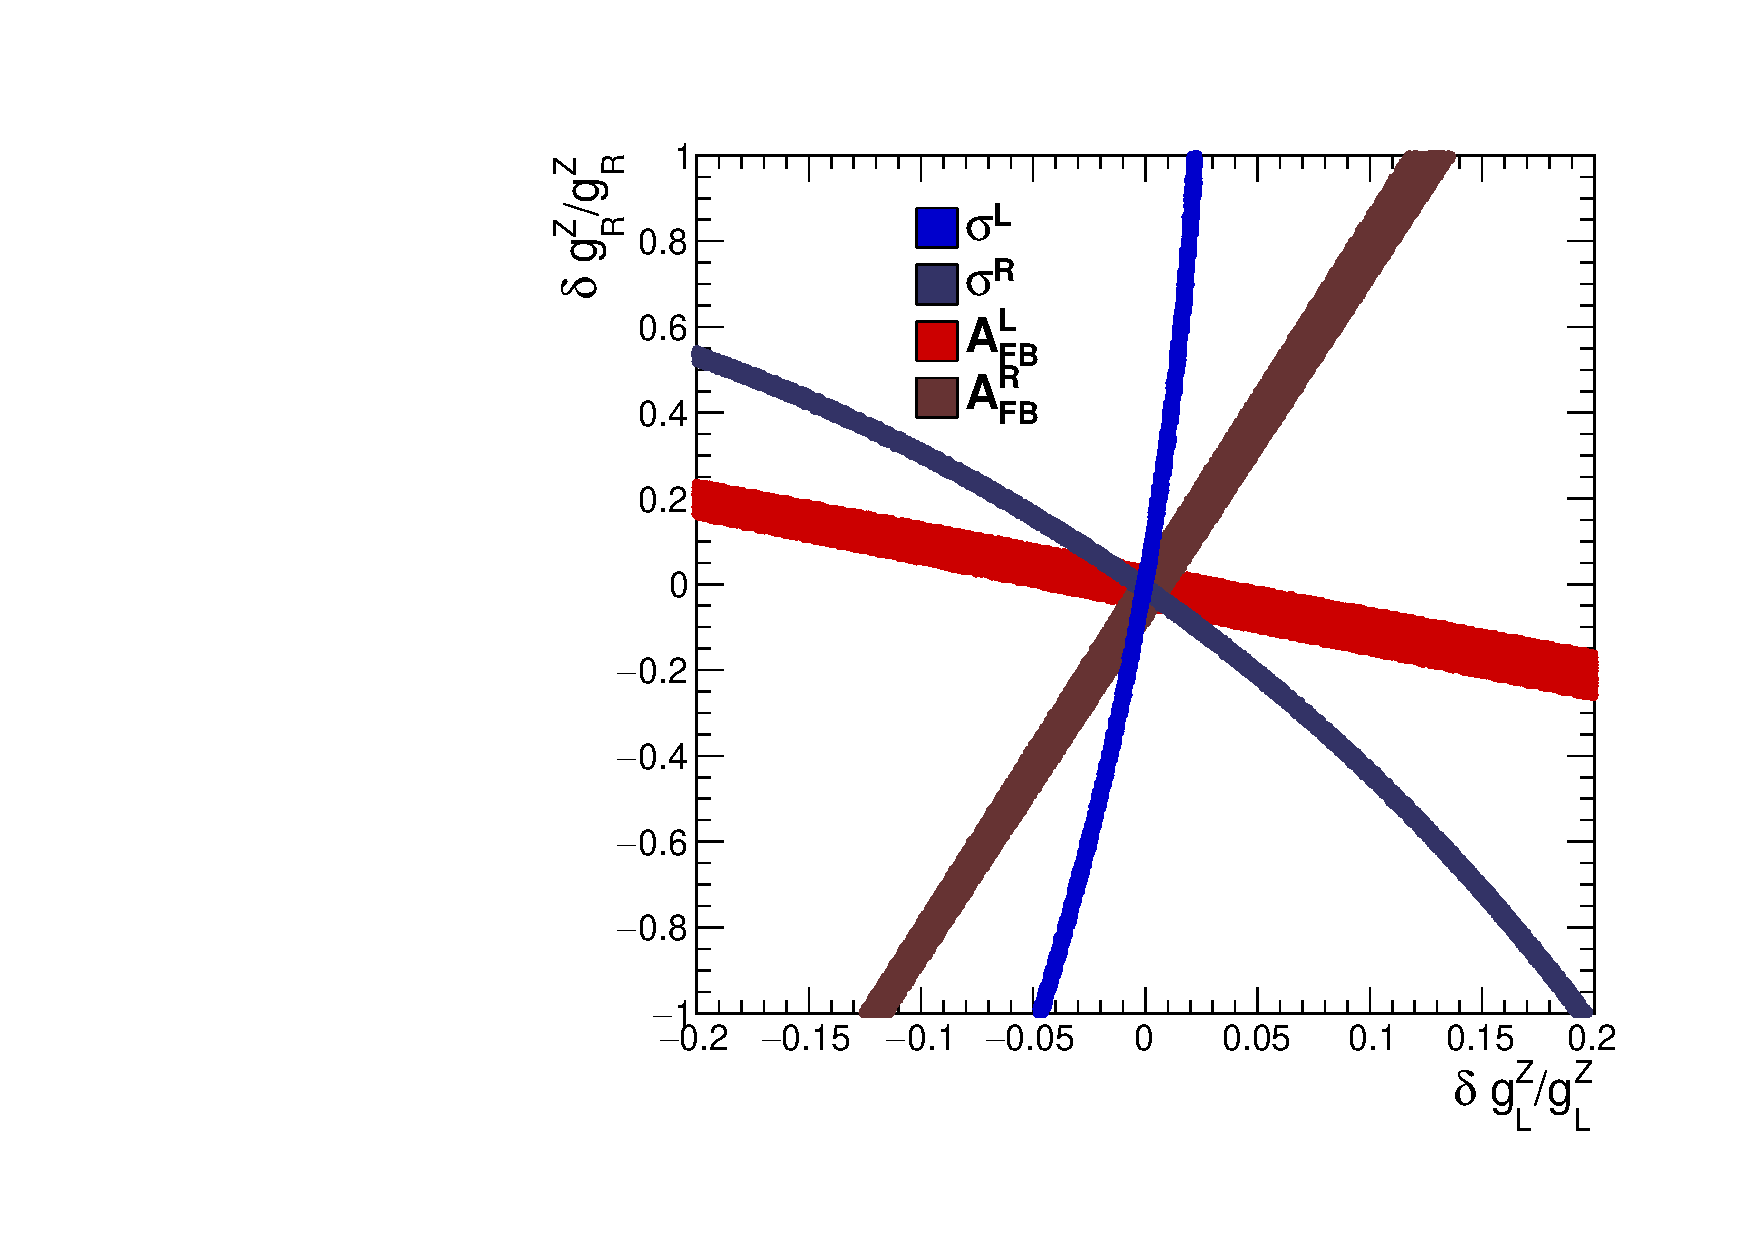
\includegraphics[width=0.99\textwidth]{ILD/plots/ilc-result.pdf}
		\caption{\label{fig:LEPILCResult_b_3F} }
	\end{subfigure}
	\caption{\sl Tree level $\pm 1\,\sigma$ allowed regions defined by the forward-backward asymmetry and total cross section measurements at LEP (a) and ILC via the differential cross section fit (b). Dashed guidelines show the \sm\ value. The allowed region expected at the ILC is centered at the \sm\ values of couplings.}
	\label{fig:LEPILCResult_3F}
\end{figure}







